% -----------------------------------------------------------------------------
%       Centro Federal de Educação Tecnológica de Minas Gerais - CEFET-MG
%
%   Modelo de trabalho acadêmico em conformidade com as normas da ABNT
%   (Tese de Doutorado, Dissertação de Mestrado ou Projeto de Qualificação)
%
%    Projeto hospedado em: https://github.com/cfgnunes/latex-cefetmg
%
%    Autores: Cristiano Fraga Guimarães Nunes <cfgnunes@gmail.com>
%             Henrique Elias Borges <henrique@lsi.cefetmg.br>
%             Denise de Souza <densouza@gmail.com>
%             Lauro César <http://www.abntex.net.br/>
% -----------------------------------------------------------------------------

\documentclass[%
    %twoside,                   % Impressão em frente (anverso) e verso
    oneside,                    % Impressão apenas no anverso
]{cefetmg}

\usepackage[%
    alf,
    abnt-emphasize=bf,
    bibjustif,
    recuo=0cm,
    abnt-doi=expand,            % Expande um endereço iniciado com doi: para http://dx.doi.org/
    abnt-url-package=url,       % Utiliza o pacote url
    abnt-refinfo=yes,           % Utiliza o estilo bibliográfico abnt-refinfo
    abnt-etal-cite=3,
    abnt-etal-list=3,
    abnt-thesis-year=final
]{abntex2cite}                  % Configura as citações bibliográficas conforme a norma ABNT

% -----------------------------------------------------------------------------
% Pacotes utilizados
% -----------------------------------------------------------------------------
\usepackage[utf8]{inputenc}                                 % Codificação do documento
\usepackage[T1]{fontenc}                                    % Seleção de código de fonte
\usepackage{booktabs}                                       % Réguas horizontais em tabelas
\usepackage{color, colortbl}                                % Controle das cores
\usepackage{float}                                          % Necessário para tabelas/figuras em ambiente multicolunas
\usepackage{graphicx}                                       % Inclusão de gráficos e figuras
\usepackage{icomma}                                         % Uso de vírgulas em expressões matemáticas
\usepackage{indentfirst}                                    % Recua o primeiro parágrafo de cada seção
\usepackage{microtype}                                      % Melhora a justificação do documento
\usepackage{multirow, array}                                % Permite tabelas com múltiplas linhas e colunas
\usepackage{subeqnarray}                                    % Permite subenumeração de equações
\usepackage{verbatim}                                       % Permite apresentar texto tal como escrito no documento, ainda que sejam comandos Latex
\usepackage{amsfonts, amssymb, amsmath}                     % Fontes e símbolos matemáticos
\usepackage[algoruled, portuguese]{algorithm2e}             % Permite escrever algoritmos em português
\usepackage[scaled]{helvet}                                 % Usa a fonte Helvetica
%\usepackage{times}                                         % Usa a fonte Times
%\usepackage{palatino}                                      % Usa a fonte Palatino
%\usepackage{lmodern}                                       % Usa a fonte Latin Modern
%\usepackage[bottom]{footmisc}                              % Mantém as notas de rodapé sempre na mesma posição
%\usepackage{ae, aecompl}                                   % Fontes de alta qualidade
%\usepackage{latexsym}                                      % Símbolos matemáticos
%\usepackage{lscape}                                        % Permite páginas em modo "paisagem"
%\usepackage{picinpar}                                      % Dispor imagens em parágrafos
%\usepackage{scalefnt}                                      % Permite redimensionar tamanho da fonte
%\usepackage{subfig}                                        % Posicionamento de figuras
%\usepackage{upgreek}                                       % Fonte letras gregas

% Redefine a fonte para uma fonte similar a Arial (fonte Helvetica)
\renewcommand*\familydefault{\sfdefault}

% -----------------------------------------------------------------------------
% Configurações de aparência do PDF final
% -----------------------------------------------------------------------------
\makeatletter
\hypersetup{%
    portuguese,
    colorlinks=true,            % true: "links" coloridos; false: "links" em caixas de texto
    linkcolor=blue,             % Define cor dos "links" internos
    citecolor=blue,             % Define cor dos "links" para as referências bibliográficas
    filecolor=blue,             % Define cor dos "links" para arquivos
    urlcolor=blue,              % Define a cor dos "hiperlinks"
    breaklinks=true,
    pdftitle={\@title},
    pdfauthor={\@author},
    pdfkeywords={abnt, latex, abntex, abntex2}
}
\makeatother

% Altera o aspecto da cor azul
\definecolor{blue}{RGB}{41,5,195}

% Redefinição de labels
\renewcommand{\algorithmautorefname}{Algoritmo}
\def\equationautorefname~#1\null{Equa\c c\~ao~(#1)\null}

% Cria o índice remissivo
\makeindex

% Hifenização de palavras que não estão no dicionário
\hyphenation{%
    qua-dros-cha-ve
    Kat-sa-gge-los
}

% -----------------------------------------------------------------------------
% Inclui os arquivos do trabalho acadêmico
% -----------------------------------------------------------------------------

% Insere e constrói alguns elementos pré-textuais para gerar capa, folha de rosto e folha de aprovação
% -----------------------------------------------------------------------------
% Capa
% -----------------------------------------------------------------------------

% -----------------------------------------------------------------------------
% ATENÇÃO:
% Caso algum campo não se aplique ao seu documento - por exemplo, em seu trabalho
% não houve coorientador - não comente o campo, apenas deixe vazio, assim: \campo{}
% -----------------------------------------------------------------------------

% -----------------------------------------------------------------------------
% Dados do trabalho acadêmico
% -----------------------------------------------------------------------------

\titulo{Análise de dados utilizand \emph{cluster} e baixo custo}
\subtitulo{tendências de consumo da
azitromicina no Brasil antes e durante a
pandemia da COVID-19}
%\title{Title in English}
\autor{Felipe Fonseca Rocha}
\local{Belo Horizonte}
\data{Julho de 2022} % Normalmente se usa apenas mês e ano

% -----------------------------------------------------------------------------
% Natureza do trabalho acadêmico
% Use apenas uma das opções: Tese (p/ Doutorado), Dissertação (p/ Mestrado) ou
% Projeto de Qualificação (p/ Mestrado ou Doutorado), Trabalho de Conclusão de
% Curso (Graduação)
% -----------------------------------------------------------------------------

\projeto{Trabalho de Conclusão de Curso II}

% -----------------------------------------------------------------------------
% Título acadêmico
% Use apenas uma das opções:
% - Se a natureza for Tese, coloque Doutor
% - Se a natureza for Dissertação, coloque Mestre
% - Se a natureza for Projeto de Qualificação, coloque Mestre ou Doutor conforme o caso
% - Se a natureza for Trabalho de Conclusão de Curso, coloque Bacharel
% -----------------------------------------------------------------------------

\tituloAcademico{Bacharel}

% -----------------------------------------------------------------------------
% Área de concentração e linha de pesquisa
% Observação: Indique o nome da área de concentração e da linha de pesquisa do Programa de Pós-graduação
% nas quais este trabalho se insere
% Se a natureza for Trabalho de Conclusão de Curso, deixe ambos os campos vazios
% -----------------------------------------------------------------------------

% \areaconcentracao{Modelagem Matemática e Computacional}
% \linhapesquisa{Sistemas Inteligentes}

% -----------------------------------------------------------------------------
% Dados da instituição
% Observação: A logomarca da instituição deve ser colocada na mesma pasta que foi colocada o documento
% principal com o nome de "logoInstituicao". O formato pode ser: pdf, jpf, eps
% Se a natureza for Trabalho de Conclusão de Curso, coloque em "programa' o nome do curso de graduação
% -----------------------------------------------------------------------------

\instituicao{Universidade Federal de Minas Gerais}
\programa{Curso de Engenharia de Sistemas}
%\programa{Curso de Engenharia de Computação}
\logoinstituicao{0.2}{./04-figuras/brasao-ufmg.jpg} % \logoinstituicao{<escala>}{<nome do arquivo>}

% -----------------------------------------------------------------------------
% Dados do(s) orientador(es)
% -----------------------------------------------------------------------------

\orientador{Ítalo Fernando Scotá Cunha}
%\orientador[Orientadora:]{Nome da orientadora}
\instOrientador{Universidade Federal de Minas Gerais}

% -----------------------------------------------------------------------------
% Folha de Rosto
% -----------------------------------------------------------------------------

% Trabalho de Conclusão de Curso
%\preambulo{{\imprimirprojeto} apresentado ao Curso de Engenharia de Computação do Centro Federal de Educação Tecnológica de Minas Gerais, como requisito parcial para a obtenção do título de {\imprimirtituloAcademico} em Engenharia de Computação.}

% Projeto de qualificação de Mestrado ou Doutorado
\preambulo{{\imprimirprojeto} apresentado ao Curso de \mbox{graduação} em Engenharia de Sistemas do Universidade Federal de Minas Gerais, como requisito parcial para a obtenção do título de {\imprimirtituloAcademico} em Engenharia de Sistemas.}

% Dissertação de Mestrado
%\preambulo{{\imprimirprojeto} apresentada ao Programa de \mbox{Pós-graduação} em Modelagem Matemática e Computacional do Centro Federal de Educação Tecnológica de Minas Gerais, como requisito parcial para a obtenção do título de {\imprimirtituloAcademico} em Modelagem Matemática e Computacional.}

% Tese de Doutorado
%\preambulo{{\imprimirprojeto} apresentada ao Programa de \mbox{Pós-graduação} em Modelagem Matemática e Computacional do Centro Federal de Educação Tecnológica de Minas Gerais, como requisito parcial para a obtenção do título de {\imprimirtituloAcademico} em Modelagem Matemática e Computacional.}

% -----------------------------------------------------------------------------
% Edite este arquivo comentando as linhas que não se aplicam ao tipo de documento acadêmico pretendido.
% -----------------------------------------------------------------------------

% -----------------------------------------------------------------------------
% Folha de Aprovação
% -----------------------------------------------------------------------------

\textopadraofolhadeaprovacao{Esta folha deverá ser substituída pela cópia digitalizada da folha de aprovação fornecida.}

% -----------------------------------------------------------------------------
% Este documento foi mantido apenas para preservar a paginação do trabalho
% acadêmico final, após a inserção da folha de aprovação fornecida
% -----------------------------------------------------------------------------


\begin{document}

% Insere os elementos pré-textuais
\pretextual
\imprimircapa                                               % Comando para imprimir Capa
\imprimirfolhaderosto{}                                     % Comando para imprimir Folha de rosto
% \imprimirfolhadeaprovacao{}                                 % Comando para imprimir Folha de aprovação
% -----------------------------------------------------------------------------
% Dedicatória
% -----------------------------------------------------------------------------

\begin{dedicatoria}

Dedico este trabalho àquela que esteve comigo na jornada dessa graduação, minha esposa. Dedico também aos meus avós, pelo suporte aos meus estudos e modelos de cidadãos e chefes de família, mas que não puderam ver a conclusão. E também aos meus pais que me incentivaram a nunca desistir.

\end{dedicatoria}
           % Dedicatória
% -----------------------------------------------------------------------------
% Agradecimentos
% -----------------------------------------------------------------------------

\begin{agradecimentos}


Agradeço a minha esposa, que em seu apoio, não só me ensinou o valor da acadêmia, mas me mostrou o papel da universidade no processo de transformação da sociedade na ostentação da tríade: ensino, pesquisa e extensão; sem nunca privilegiar um em detrimento do outro.

Ao meu orientador, Prof. Dr. Ítalo Fernando Scotá Cunha pela ajuda durante o processo de formulação de um trabalho válido e suas contribuições a este.

Aos docentes exemplares do curso de Engenharia de Sistemas, que em muito contribuíram para minha formação.

À Prof. Dra. Ana Liddy Cenni de Castro Magalhães, por sua excelente coordenação e o secretário do Colegiado de Engenharia de Sistemas, Júlio César Pereira de Carvalho, por sua disponibilidade e suporte.

Ao Centro de Estudos de Medicamentos da Faculdade de Farmácia da UFMG e todos os seus membros, por sua iluminação sobre o que é a extensão aliada ao ensino e orientada a pesquisa.

Aos colegas do curso que dividiram seus conhecimento e experiências.

A minha família, pela força motriz de tudo o que construo.

Aos meus amigos, dentre eles graduados, mestres e doutores pela sua importância ao longo da minha trajetória.

\end{agradecimentos}
        % Agradecimentos
% -----------------------------------------------------------------------------
% Epígrafe
% -----------------------------------------------------------------------------

\begin{epigrafe}

\emph{''Os livro têm muita coisa escrita, é o que ele diz}

\emph{Em pleno berço de Machado de Assis, olha o que eu sou obrigado a ouvir}

\emph{Nega a ciência, esconde a doença, só negligência}

\emph{Essa é a sentença pra falta de consciência que colocou ele ali''}

(Chico César, DJ Caique, Rashid, Diário de Bordo 6)

\end{epigrafe}

% -----------------------------------------------------------------------------
% Edite o texto acima para inserir uma epígrafe de sua preferência
% -----------------------------------------------------------------------------
              % Epígrafe
% -----------------------------------------------------------------------------
% Resumo
% -----------------------------------------------------------------------------

\begin{resumo}
    Análise de grandes massas de dados, por vezes requer um, ou mais computadores de alto desempenho para tornar viável a extração de informações. Na área da pesquisa, principalmente de instituições publicas, há uma restrição orçamentaria que nos últimos anos apresentou uma diminuição do valor disponibilizado. Dessa forma, áreas de estudo, como a da saúde, que possuem um volume de dados considerável, vêm enfrentando problemas na aquisição desses equipamentos que habilitam essas análises. Uma alternativa a necessidade de computadores de auto desempenho é o uso de técnicas de computação distribuída. O objetivo deste trabalho visa realizar o estudo das ferramentas disponíveis no mercado e propor uma solução de implementação e comparação, para no trabalho posterior, comparar o desempenho de orquestração de recursos em \emph{cluster} de baixo custo em ambientes com virtualização completa e virtualização baseada em contêineres para o processamento e a análise de dados em saúde, como tendência de consumo de azitromicina entre os anos 2014 e 2021. Ainda nesse trabalho apresenta-se uma avaliação de impactos econômicos na processamento de dados e aspectos sociais de contribuição resultantes dessa pesquisa.
    % A comparação entre os dois tipos de virtualização, por meio da taxa de utilização de memória e processamento, além do tempo de execução indicarão qual estratégia mais viável para composição do \emph{cluster}. E poderão ser comparados com a excussão em um computador com a soma dos recursos computacionais do cluster.

    \textbf{Palavras-chave}: Kubernetes\textregistered. Virtualização. Contêineres. Hypervisor Tipo 2. Análise de dados.
\end{resumo}

% -----------------------------------------------------------------------------
% Escolha de 3 a 6 palavras ou termos que descrevam bem o seu trabalho. As palavras-chaves são utilizadas para indexação.
% A letra inicial de cada palavra deve estar em maiúsculas. As palavras-chave são separadas por ponto.
% -----------------------------------------------------------------------------
             % Resumo na língua vernácula
% -----------------------------------------------------------------------------
% Abstract
% -----------------------------------------------------------------------------

\begin{resumo}[Abstract]
    The analysis of large volumes of data sometimes requires one or more high-performance computers to make extracting information viable. In the research's area, mainly in public institutions, there is a budget constraint that, in recent years, has shown a growing decrease in available resources, making it impossible to acquire computers that allow such analyses. An alternative to the need for high-performance computers is the use of distributed computing techniques. Thus, the orchestration of Kubernetes\textregistered\ clustered resources was performed for data processing and analysis. In addition, the feasibility of this solution was evaluated in terms of performance, complexity and economic viability, having as a workload the analysis of azithromycin consumption data, in Brazil, between the years 2014 and 2020. Eight computers were used in the structuring the cluster, adding up to 42 CPUs and 88 GB RAM. For ease of configuration, while keeping the clusters secure, they were all configured with SSH keys for remote access. The use of desktops in the composition of the cluster - which will continue to be available for use in the Department of Computer Science - made it possible to process more than 70 GB of data in a distributed manner, in 53 minutes, without any additional cost with the acquisition of equipment for analysis of data. Regarding the data on azithromycin consumption, in Brazil, an increase in prescription rates per 1,000 inhabitants was observed over the time series from 66.2 to 83.8 prescriptions, as well as in almost all federative units, with emphasis on Minas Gerais (66.2 to 149.2 prescriptions per 1,000 inhabitants), Rondônia (37.5 to 109.4 prescriptions per 1,000 inhabitants) and Roraima (37.2 to 99.8 prescriptions per 1,000 inhabitants). A similar behavior was also observed, in the comparative analysis between the years before and during the pandemic (2019 and 2020), with an increase from 59.9 to 83.8 prescriptions per thousand inhabitants, in the country. The accomplishment of this work showed that the use of Kubernetes\textregistered\ cluster is a promising alternative for analyzing large volumes of data, especially from the point of view of using underutilized resources, with the recruitment process through dynamic configuration of configuration managers. And that, considering the data analyzed, apparently the COVID-19 pandemic - including the disclosure of azithromycin in COVID kits - may have influenced the greater increase in the consumption of this drug.


    \textbf{Keywords}: Kubernetes. Virtualization. Containers. Hypervisor Type 2. Data analysis.
\end{resumo}

% -----------------------------------------------------------------------------
% O restante da formatação deve manter-se igual ao do resumo em português, i.e, um único parágrafo.
% -----------------------------------------------------------------------------
             % Resumo em língua inglesa
% -----------------------------------------------------------------------------
% Lista de Figuras
% -----------------------------------------------------------------------------

\pdfbookmark[0]{\listfigurename}{lof}
\listoffigures*
\cleardoublepage

% -----------------------------------------------------------------------------
% Este arquivo não necessita de ser editado. A lista é gerada automaticamente.
% -----------------------------------------------------------------------------
         % Lista de figuras
% -----------------------------------------------------------------------------
% Lista de Tabelas
% -----------------------------------------------------------------------------

\pdfbookmark[0]{\listtablename}{lot}
\listoftables*
\cleardoublepage

% -----------------------------------------------------------------------------
% Este arquivo não necessita de ser editado. A lista é gerada automaticamente.
% -----------------------------------------------------------------------------
         % Lista de tabelas
% % -----------------------------------------------------------------------------
% Lista de Quadros
% -----------------------------------------------------------------------------

\pdfbookmark[0]{\listofquadrosname}{loq}
\listofquadros*
\cleardoublepage

% -----------------------------------------------------------------------------
% Este arquivo não necessita de ser editado. A lista é gerada automaticamente.
% -----------------------------------------------------------------------------
         % Lista de quadros
% % -----------------------------------------------------------------------------
% Lista de Algoritmos
% -----------------------------------------------------------------------------

\newcommand{\algoritmoname}{Algoritmo}
\renewcommand{\listalgorithmcfname}{Lista de Algoritmos}

\floatname{algocf}{\algoritmoname}
\newlistof{listofalgoritmos}{loa}{\listalgoritmoname}
\newlistentry{algocf}{loa}{0}

\counterwithout{algocf}{chapter}
\renewcommand{\cftalgocfname}{\algoritmoname\space}
\renewcommand*{\cftalgocfaftersnum}{\hfill--\hfill}

\pdfbookmark[0]{\listalgorithmcfname}{loa}
\listofalgorithms
\cleardoublepage

% -----------------------------------------------------------------------------
% Este arquivo não necessita de ser editado. A lista é gerada automaticamente.
% -----------------------------------------------------------------------------
      % Lista de algoritmos
% % -----------------------------------------------------------------------------
% Lista de Siglas
% -----------------------------------------------------------------------------

\begin{siglas}
    \item[ABNT] Associação Brasileira de Normas Técnicas
    \item[DECOM] Departamento de Computação
\end{siglas}

% -----------------------------------------------------------------------------
% Edite a lista acima para definir "todos" os acrônimos e siglas utilizados neste trabalho
% -----------------------------------------------------------------------------
          % Lista de abreviaturas e siglas
% % -----------------------------------------------------------------------------
% Lista de Símbolos
% -----------------------------------------------------------------------------

\begin{simbolos}
    \item[$ \Gamma $] Letra grega Gama
    \item[$ \lambda $] Comprimento de onda
    \item[$ \in $] Pertence
\end{simbolos}

% -----------------------------------------------------------------------------
% Edite a lista acima para definir "todos" os símbolos utilizados neste trabalho
% -----------------------------------------------------------------------------
        % Lista de símbolos
% -----------------------------------------------------------------------------
% Sumário
% -----------------------------------------------------------------------------

\pdfbookmark[0]{\contentsname}{toc}
\tableofcontents*
\cleardoublepage

% -----------------------------------------------------------------------------
% Este arquivo não necessita de ser editado. O sumário é gerado automaticamente.
% -----------------------------------------------------------------------------
               % Sumário

% Insere os elementos textuais
\textual
% -----------------------------------------------------------------------------
% Introdução
% -----------------------------------------------------------------------------

\chapter{Introdução}
\label{chap:introducao}

\section{Motivação}
\label{sec:motivacao}

No contexto da análise de dados, diferentes ferramentas estão disponíveis para transformá-los em informação, contudo o uso dessas ferramentas na área da saúde ainda é pouco significativo \cite{galvao_desafios_2019}. Frente a uma tendência crescente de interconexão entre diferentes áreas do conhecimento e do potencial que a análise de dados possibilita para melhoria do sistema de saúde, se faz necessário propor e validar estratégias que permitam o avanço na integração de dados entre diferentes Sistemas de Informação em Saúde (SIS), e que facilitem o processamento e análise do grande volume de dados produzidos e disponibilizados nesses sistemas \cite{galvao_desafios_2019,mehta_concurrence_2018}.

Atualmente, conforme determinação do Decreto nº 8.777, de 11 de maio de 2016, que instituiu a Política de Dados Abertos do Poder Executivo Federal \cite{brasildisponibilidade2016}, diversos dados dos SIS são disponibilizados de forma pública. No entanto, apenas a disponibilização dos dados em si não garante que eles poderão ser analisados visando produzir informação relevante para as políticas públicas na área da saúde.

\section{Justificativa}
\label{sec:justificativa}


Alterações de governo e vertentes políticas mudam as prioridades de investimento e interesses o que faz com que o orçamento de alguns pilares de investimento e custo no país flutue como observado nos últimos 10 anos (Tabela \ref{tab:orcamento}). A disponibilidade de recursos financeiros efetivos para a ciência e tecnologia no Brasil têm oscilado. Nos anos de 2018 a 2021 sofreu reduções acentuadas, o que tornou ainda mais limitado o acesso a recursos que viabilizem a realização de análise dos dados em ferramentas e infra estruturas tradicionais ou ainda a proposta de novos.

Em uma avaliação simples desses dados, somado a variação do valor do dólar no mesmo periodo pode se observar (Figura \ref{fig:dolar}), pode ser ver um aumento de mais de $327\%$. Sendo que o orçamento não acompanhou essa flutuação. Essa ligação, apesar de não ser direta existe, sendo que em ciência e tecnologia equipamentos, licenças de \emph{software} etc utilizados no processamento de dados, são majoritariamente importadas, e portanto em dólar. Como o valor do orçamento efetivo por ano não acompanha o aumento do dólar, fica claro a perda de poder de compra, dado que a distribuição de verba do orçamento total tenha se mantido. 

Algo que valida a flutuação orçamentária é a queda consecutiva de orçamento desde 2018 (Figura \ref{fig:quedaorca}). Ainda podemos entender que mesmo em depois de 10 anos, temos um orçamento $2,32\%$ menor para ciência e tecnologia, o que impacta diretamente no financiamento de novos projetos, especialmente na compra de equipamentos que viabilizam pesquisas de larga escala ou que se valem de bases muito grandes como é o caso de bases como DataSUS e os diversos sistemas que compõem e, também, o banco de repasse orçamentário, limitando apenas para SUS, vindo de outras fontes como orçamento da união com pagamento diário e/ou semanal. Sem o poder computacional a disposição para estudo desses bancos, principalmente em instituições públicas, fica inviável a produção de conhecimento, a audição pela população e qualquer extração de informação viável. 

Essas limitações indiretas, impõem forte restrições no processo de avaliação e tomada de decisão embasada em dados. Ainda avaliando esse impacto econômico do problema descrito acima, é preciso pensar, como já discutido, a complexidade de tomada de decisões em saúde. Sem informações que embasem essa decisão fica restrita a capacidade de compreensão do senário nacional, sobre a situação de saúde pública. Quando leva-se em consideração que o SUS é um sistema subfinanciado, quando comparado a países que também possuem sistemas de saúde pública e gratuitas. O valor do orçamento por dia por pessoa é de apenas $R\$ 3,83$  o que é um preceito quando considera-se  restrição orçamentária do SUS por pessoa. Para entender a complexidade de um sistema tão abrangente é preciso avaliar sua escala. Mais de 152 milhões de pessoas utilizam exclusivamente o SUS como promotor de saúde. 

\begin{table}[htpb]
\centering
  \caption{Pagamento efetivo - Ministério da Ciência e Tecnologia}
  \label{tab:orcamento}
  \begin{tabular}{cc}
    \hline
    \textbf{Ano} & \textbf{Objetivo}    \\
    \hline
    2010         & R\$ 6.288.931.123,00 \\
    2011         & R\$ 5.918.584.706,00 \\
    2012         & R\$ 6.918.288.201,00 \\
    2013         & R\$ 7.787.464.592,00 \\
    2014         & R\$ 8.598.785.224,00 \\
    2015         & R\$ 7.964.319.815,00 \\
    2016         & R\$ 8.404.014.691,00 \\
    2017         & R\$ 9.085.620.227,00 \\
    2018         & R\$ 9.157.748.260,00 \\
    2019         & R\$ 8.812.096.752,00 \\
    2020         & R\$ 7.859.851.948,00 \\
    2021         & R\$ 6.142.873.884,00
  \end{tabular}
  \centering
  \begin{tablenotes}
  \centering
    \small
    \item{Fonte: SIOP consulta realizada em Janeiro de 2022}
  \end{tablenotes}
\end{table}

\begin{figure}[!h]
    \centering
    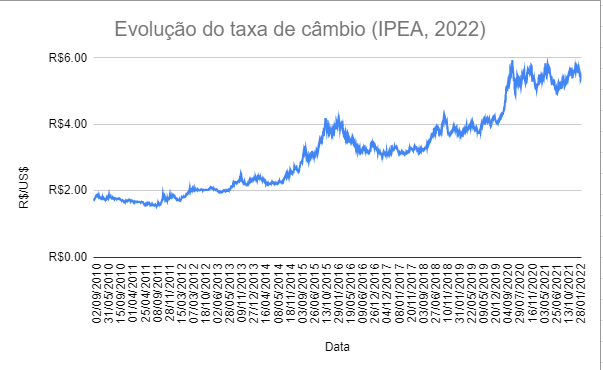
\includegraphics[width=0.8\textwidth]{04-figuras/dolar.png}
    \caption[Evolução do dólar/real na última década ]{Evolução do dólar/real na última década (Fonte: Feito pelo autor)}
    \label{fig:dolar}
\end{figure}
\begin{figure}[!h]
    \centering
    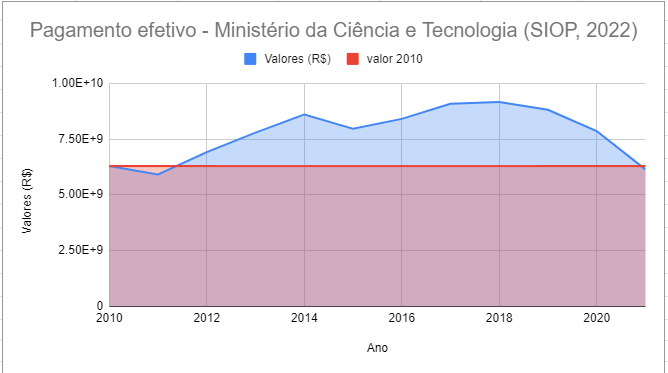
\includegraphics[width=0.8\textwidth]{04-figuras/compartive.png}
    \caption[Pagamento efetivo - Ministério da Ciência e Tecnologia ]{Pagamento efetivo - Ministério da Ciência e Tecnologia (Fonte: Feito pelo autor)}
    \label{fig:quedaorca1}
\end{figure}
\begin{figure}[!h]
    \centering
    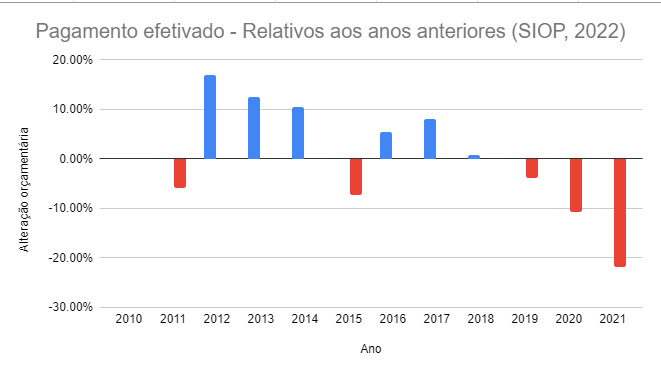
\includegraphics[width=0.8\textwidth]{04-figuras/compartive_last .png}
    \caption[Pagamento efetivo - Relativos aos anos anteriores ]{Pagamento efetivo - Relativos aos anos anteriores (Fonte: Feito pelo autor)}
    \label{fig:quedaorca}
\end{figure}

Tendo dado o contexto desse impacto na economia bem como na sociedade o presente trabalho se propõe a discutir alternativas e abordagens que amenizem impactos de orçamento disponibilizados pelo governo durante a viabilização de projetos de pesquisa que utilizam bases de dados tão grandes.

Nesse sentido, temos dois efeitos diretos:

\begin{itemize}
    \item Redução de fragilidade orçamentária
    \item Proposta de alternativas para análise de dados em saúde
\end{itemize}

A redução de fragilidade orçamentária se dá pela proposta de utilização de recursos já disponíveis e subutilizados, como \emph{desktops} de bibliotecas, laboratórios etc, por meio de ambientes virtualizados, compartilhando esses recursos com a orquestração das cargas de trabalhos de análise de dados. Para viabilizar essa proposta, o trabalho compara a performance de sistemas virtuais em computadores com baixo poder computacional, propondo assim uma forma de abordar, tanto o isolamento, para processos mais sensíveis, quanto a utilizam de recursos que já estão disponíveis o que garante o menor CAPEX possível para excussão do projeto de pesquisa. 

Para avaliação dessa alternativa toma-se como exemplo os bancos de “Vendas de Medicamentos Controlados e Antimicrobianos - Medicamentos Industrializados”, objeto deste trabalho, estão disponíveis cerca de 70 GB e com mais de 500 milhões de linhas de dados sobre a comercialização de medicamentos no país. Logo, tão importante quanto a disponibilidade pública dos dados, é fundamental encontrar estratégias técnicas e economicamente viáveis a fim de possibilitar que pesquisadores em todo o país possam contribuir com a análise e a interpretação desses dados, mesmo frente a baixa disponibilidade de recursos financeiros e de infraestrutura, como servidores de alta performance (HPC), por exemplo.

\section{Objetivos}
\label{sec:objetivos}
Diante disso, com a realização deste trabalho espera-se oferecer uma alternativa para análise de grandes volumes de dados que possua baixo custo financeiro, menor complexidade de configuração, maior efetividade (menor tempo de análise) e que não seja dependente da disponibilidade ou uso de recursos dedicados, como computadores de alta performance (HPC), às análises. A abordagem que irá se seguir é na utilização de alternativas \emph{open source} atualmente disponíveis que seja possíveis de serem utilizadas em computadores de baixo custo e menor poder computacional - ex.: \emph{OpenStack}, \emph{CloudStack} etc.

Deste modo, espera-se demonstrar comparativamente a implementação de uma solução para análise de dados em plataformas de orquestração de \emph{containers}, que permita recrutar computadores comuns para essa análise. E assim, espera-se, superar de maneira custo-efetiva um problema de restrição orçamentária e técnica para instituições públicas e grupos de pesquisa que realizam análises de grande volumes de dados. No caso deste trabalho, a aplicação está direcionada para a área da saúde, utilizando uma tecnologia já amplamente empregada no setor privado, o que viabiliza o suporte de estudantes e/ou profissionais das áreas de Engenharias e Computação. Espera-se, ainda, contribuir para que os dados públicos em saúde sejam analisados com  maior frequência e menor restrição, gerando indicadores melhores e atualizados para melhor tomada de decisão em saúde.

\section{Definição e abordagem}
\label{sec:abordagem}

A proposta do trabalho visa avaliar a utilização de \emph{cluster} de Kubernetes\textregistered \ como plataforma de orquestração de cargas de trabalho para processamento de dados em \emph{clusters }compostos por computadores de baixo custo ou reaproveitados.

Utilizando como carga de trabalho a análise de tendência de consumo de azitromicina no Brasil entre os anos de 2014 e 2021. Pretende-se utilizar, como principal resultado, a viabilidade de utilização de computadores do tipo \emph{desktop} para orquestração e análise de grades massas de dados como dados do SUS (Sistema Único de Saúde) garantindo assim viabilidade de trabalhos e proponto a utilização dessa plataforma em computadores menos específicos, como alternativa a HPC.

A utilização da plataforma visa validar seu uso para orquestração de tarefas em paralelo e precessamneto distribuído de dados, durante a análise, permitindo o uso simultâneo de diversas máquinas. Utilizando inicialmente 8 computadores com capacidades de processamento semelhantes a computadores desktop de 8-16 GB (Gigabytes) de RAM (Random Access Memory) e 4-8 vCPU (virtual Central Process Unit). Essa restrição  permitiram que uma análise de viabilidade para que o processmaneto e análise de grandes massas de dados (maiores que 50 GB) possam ser feitas sem o uso de HPC.

A abordagem de DevOps (BASS et al, 2015) para tornar o provisionamento, a integração e o \emph{deploy} da infra estrutura, bem como os componentes de análise desses utilizados neste trabalho incluem o conceito de CI (continuous integration), CD (continuous delivery).  IaC (Infrastructure as Code) visa tornar a configuração e disponibilização desse \emph{cluster} mais ágil, diminuindo assim a necessidade de operação e também de sua manutenção.

Para a análise de dados utilizando a estratégia descrita, propõe-se analisar as tendências de consumo da azitromicina no período de 2014 a 2021. Essa análise é objeto de carga de trabalho a ser orquestrado de maneira distribuída no \emph{cluster} para validação de seu desempenho nos ambientes propostos.

O trabalho não engloba a realização de interpretação da informação gerada pelo banco, garantindo, assim, apenas o resultado correto da análise citada como carga de trabalho para comparação. Também não está sendo proposta uma metodologia de análise do banco referenciado, mas a avaliação das tecnologias empregadas para orquestração das tarefas, comparação de desempenho entre as alternativas da implementação da plataforma e sua implementação como proposta para uso mais amplo nas instituições sob restrição orçamentária, com o fim de continuar a realizar análises de dados, ainda que sem hardware adequado.


\section{Organização do trabalho}
\label{sec:organizacaoTrabalho}

Este trabalho está dividido em 5 Capítulos. Esta Introdução apresentou o contexto geral do trabalho e tecnologias que serão avalias e citou possíveis problemáticas econômicas e sociais. 

O Capítulo 2 apresenta a fundamentação teórica e a revisão da literatura, discorrendo sobre as leituras que embasaram toda a construção do projeto, também aprofunda em conceitos necessários para as discussão e condução do trabalho. 

O Capítulo 3 apresenta a  metodologia utilizada para a construção dos componentes do projeto e a forma de avaliação de desempenho dos ambientes propostos bem como a forma de avaliação. 

O capitulo \ref{ch} apresenta os resultados obitidos tanto para orquestração das cargas de trabalho no ETL (extração, transformação e carga) e também os resultados obtidios apara a análise e processamento dos dados de consumo e prescrição obtidos para azitromicina no periodo descrito anteriormente.
discute os resultados adquiridos para a orequestração e análise dos dados de prescrição da azitromicia, além de suas interprestações. 

O capítulo \ref{chap:conclusao} apresenta as conclusões até a finalização do trabalho, discorre sobre as fases do TCC e também apresenta o que o aluno realizou ao longo da execução do trabalho, se a proposta do trabalho atingiu a espectativa como solução ao problema  proposto, além de possibilidades para trabalhos futuros.                 % Introdução
% % -----------------------------------------------------------------------------
% Trabalhos Relacionados
% -----------------------------------------------------------------------------

\chapter{Trabalhos Relacionados}
\label{chap:trabRelac}

Cada capítulo deve conter uma pequena introdução (tipicamente, um ou dois parágrafos), em seção não numerada, que deve deixar claro o objetivo e o que será discutido no capítulo, bem como a organização do capítulo.
    % Trabalhos relacionados
% -----------------------------------------------------------------------------
% Fundamentação Teórica
% -----------------------------------------------------------------------------

\chapter{Fundamentação Teórica}
\label{chap:fundamentacaoTeorica}

\section{Análise de dados em saúde}

A tomada de decisões em saúde precisa com frequência do suporte de um profissional especializado na temática a ser decidida. Uma série de técnicas são aplicadas por esse profissional para avaliação do contexto, uma vez que os dados puros não são suficientes, devido à multifatoriedade \cite{andrade_tomada_2008,resende2009}. O grande número de sistemas de auxílio em saúde, sejam esses de ordem regulatória ou ainda por iniciativas privadas, fazem com que o volume de dados cresça exponencialmente, produzindo o fenômeno de \emph{Big Data}. Uma definição conhecida desse conceito aponta volume, variedade e velocidade como os três vetores relacionados à produção massiva de dados \cite{laney20013d}. Outras características foram adicionadas a essa primeira definição de\emph{Big Data}, tais como veracidade \cite{schroeck2012analytics},  complexidade e desestruturação \cite{intel2012}, e valor \cite{oracle2013}.

A multifatoriedade já citada é um aspecto que se relaciona à complexidade dos dados em grande volumes. É cada vez mais difícil estabelecer uma relação de causa e efeito para a tomada de decisão segura, sem auxílio ou sumarização desses dados em informações mais tangíveis e associadas. Também é difícil descrever um algoritmo que permita analisar todos os dados de contexto e relacioná-los de forma que possa ser utilizado como substituição ao conhecimento tácito de um profissional da saúde experiente \cite{faceli2011}.

O suporte de sistemas, métodos e pŕaticas que auxiliem a assistência em saúde no tratamento de \emph{Big Data}  ainda não é suficientemente consolidado. Faltam evidências de aplicações especialmente quantitativas que validem seu uso nesse campo do conhecimento. Além disso, boa parte das tecnologias utilizadas nesses estudo estudos, utilizam recursos específicos de computação e frequentemente esses recursos têm custo elevado. Esses estudo focam na  avaliação de dados para otimização de recursos, suporte a decisões clínicas e redução de custo do cuidado \cite{nishita2018} e não na análise de dados para tomadas de decisão em saúde pública, nem tão pouco no auxílio para construção de politicas públicas. Ambos os focos são válidos, porém apresentam conceitos distintos e a forma de extrair essas informações são diferentes.

Há uma grande oportunidade de estudo na proposição de um \emph{stacks} (conjunto de ferramentas) e métodos para extrair essas informações no contexto de saúde pública. O desenvolvimento de abordagens para o processamento de dados nesse contexto de estudo pode viabilizar a utilização de grandes bases de dados públicas o que permitiria o estabelecimento de novas correlações e posteriormente associação com demais bancos, ou conjuntos de informações.

Sendo o paragrafo acima, justamente o que esse trabalho se propõe, ainda que o volume de dados da base sob análise neste trabalho e sua composição não qualifiquem como \emph{Big data}, sob a perspectiva de LANEY. Esse trabalho pode ser utilizado de base para uma nova forma de utilização de recursos computacionais na análise de grandes massas de dados e a posteriori \emph{Big Data}. 

\section{Virtualização}
Virtualização, no contexto de computação, é refere se à abstração de componentes e/ou recursos de computador. O objetivo do ambiente de computação virtual é melhorar a utilização de recursos, por meio da utilização sob demanda destes recursos, sendo essa demanda a forma de utilização e a quantidade de recursos necessários. Virtualização fornece uma plataforma operacional unificada e integrada para usuários e aplicativos com base na agregação de recursos heterogêneos e autônomos.

Essa abstração é, usualmente, feita por uma camada de software entre \emph{hardware} e SO (SO), chamada de \emph{hypervisor} ou monitor de maquina virtual (VMM).

Mais recentemente, a virtualização em todos os níveis (sistema, armazenamento e rede) tornou-se importante novamente como forma de melhorar a segurança, confiabilidade e disponibilidade do sistema, reduzir custos e fornecer maior flexibilidade.\cite{virt}

Existem diversos níveis de abstração para virtualização, considerando níveis mais detalhados de funcionalidades e/ou níveis menos específicos de hardware. Isso torna possível extrair aplicações e seus respectivos ambientes com mais facilidade e troca-los de máquina base, considerando essa mudança como portabilidade. Como objeto de estudo deste trabalho nos limitamos a definição de dois tipos de virtualização: completa, nível de SO.

\subsection{Virtualização completa}

Virtualização completa, sendo intermediada por sistema s VMM ou \emph{hypervisor} também é chamado de máquina virtual gerenciador e é executado em cima de um SO \emph{host}, geralmente como um aplicativo no SO base. O resultado é que, nas VMs, os aplicativos e o SO convidado são executados em cima de um hardware virtual fornecido pelo \emph{hypervisor}. Pode ser considerado para fornecer "Virtualização Completa".

Neste tipo de configuração, os dispositivos de E/S são atribuídos às máquinas convidadas (\emph{guest}), imitando os dispositivos físicos. A interação com esses dispositivos no ambiente virtual são então direcionados para os dispositivos físicos reais, seja pelo \emph{driver} do SO do host ou pelo "\emph{Driver VM}". 

Essa arquitetura pode ser observada na Figura \ref{fig:vms}. A principal vantagem dessa abordagem é que é muito fácil de usar. Um usuário comum pode instalar um produto de software como o \textregistered{VirtualBox} como qualquer outro produto de software no SO de sua escolha. Dentro do deste virtualizador, um SO \emph{guest} pode ser instalado e usado como se estivesse sendo executado diretamente no hardware. \cite{portnoy2012virtualization}

\begin{figure}[!h]
    \centering
    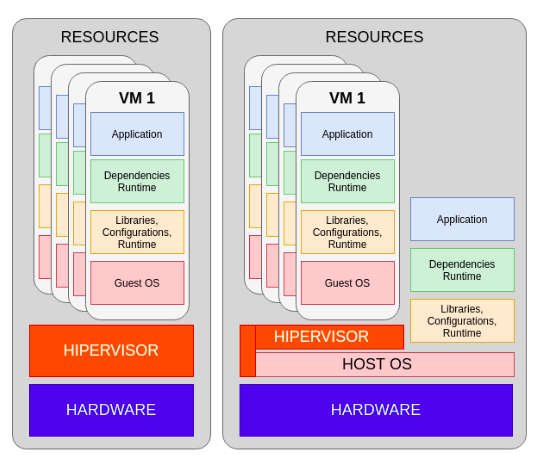
\includegraphics[width=0.8\textwidth]{04-figuras/vms.png}
    \caption[Hosted \emph{hypervisor} diagrama representativo de componentes ]{Hosted \emph{hypervisor} diagrama representativo de componentes (Fonte: Google Images, 2021)}
    \label{fig:vms}
\end{figure}

\subsection{Containers ou virtualização em nível de SO}

Conhecida também como \emph{container}, é uma técnica de virtualização que referece ao uso compartilhado do kernel do SO, porém manipula a forma de execução dos processo no \emph{userspace}, setando dois conjuntos de configurações, \emph{namespace} (isolamento dos recursos de sistema) e \emph{cgroup} (controle de utilização dos recursos).

\cite{redhat2018}
\subsubsection{Container}
\emph{Containers} são um conjunto de 1 ou mais processos sendo executados isolados do sistema base.

\subsubsection{Runtime}
Como no \emph{hypervisor} que executa e comunica com o sistema base ou hardware, para \emph{container} tempos o \emph{container} \emph{runtime} que é responsável por executar o \emph{container} e gerenciar o namespace e gcgroups definido para aquele \emph{container}.

\subsubsection{Orquestrator}
O orquestrador de \emph{container} é sistema responsável por avaliar e comandar a execussão dos \emph{container} por meio do \emph{runtime}, tendo como premissa a disponibilização dos recursos totais da maquina e garantindo que o \emph{container} esteja executando de acordo com uma  serie de parametros, bem como também é responsável pelas configurações de rede que serão utilizadas e gerenciadas ao logo do ciclo de vida dos \emph{container}s sob sua orquestração.

\section{Alternativas open source}

Para avaliar alternativas no mercado a seguinte estratégia de pesquisa foi conduzinda nas seguintes bases:

\begin{itemize}
    \item IEEE Xplore
    \item \emph{Computers and Applied Sciences Complete}
\end{itemize}

\subsection{Termos consultados}
Para organizar os termos selecionados para a busca, bem como a suas variações de consulta foi realizada uma agrupamento de palavras em temas e utilizadas combinações de termos de cada tema segundo a estrutura apresentada na tabela \ref{table:termos}.

A formatação da estratégia de pesquisa esta contida nas tabelas \ref{table:ieee} e \ref{table:computing}. Essa formatação permite indicar estudos que tenham os temas indicados de forma reduzida por assunto, título, palavras chave e resumo e a partir dessa extração, uma avaliação de ferramentas utilizadas resultou no levantamento de tecnologias a serem avaliadas na próxima sessão. Levando em consideração um filtro adicional que é ser \emph{Open Source}.

\begin{center}
\begin{table}[!htbp]
\begin{tabular}{cccc}
\textbf{CLUSTER}                                                  & \textbf{DATA PROCESSING}                                                                              & \textbf{COST}                                                                                                    & \textbf{COMPUTING}                                                                                                                               \\ \hline
\begin{tabular}[c]{@{}c@{}}cluster\\ “small cluster”\end{tabular} & \begin{tabular}[c]{@{}c@{}}“data process”\\ “data processing”\\ “data processing system”\end{tabular} & \begin{tabular}[c]{@{}c@{}}cost\\ “low cost”\\ “lowest cost”\\ “cheap”\\ “economic”\\ “inexpensive”\end{tabular} & \begin{tabular}[c]{@{}c@{}}computing\\ “grid computing”\\ “mist computing”\\ “cloud computing”\\ “fog computing”\\ “edge computing”\end{tabular} \\ \hline
\begin{tabular}[c]{@{}c@{}}\#1 Combinar \\ OR\end{tabular} & \begin{tabular}[c]{@{}c@{}}\#2 Combinar \\ OR\end{tabular} & \begin{tabular}[c]{@{}c@{}}\#4 Combinar \\ OR\end{tabular}                                                       & \#6 Combinar com OR \\ \hline
\multicolumn{1}{l}{} & \#3 \#1 AND \#2 & \#5 \#3 AND \#4 & \#7 \#5 AND \#6                                                                                                                                  \\ \hline
\end{tabular}
\caption{Termos de pesquisa e estratégia de agrupamento}
\label{table:termos}
\end{table}
\end{center}


\begin{table}[!htbp]
\centering
\begin{tabular}{ccc}
\textbf{Passo} & \multicolumn{1}{c}{\textbf{Operação}}                                                                                                                                               & \textbf{Resultados}  \\ \hline
\textbf{\#1}   & \begin{tabular}[c]{@{}l@{}}$$ALL = (\\ \ \ \ \ cluster\\ \ \ \ \ OR "small cluster"\\ )$$\end{tabular}  & 1.199.979  \\ \hline
\textbf{\#2}   & \begin{tabular}[c]{@{}l@{}}$$ALL = (\\ \ \ \ \ “data process” \\  \ \ \ \ OR “data processing” \\  \ \ \ \ OR “data processing system”\\ )$$\end{tabular} & 88.988  \\ \hline
\textbf{\#3}   & \#1 AND \#2 & 5.810  \\ \hline
\textbf{\#4}   & \begin{tabular}[c]{@{}l@{}}$$ALL = (\\  \ \ \ \ “low cost” \\  \ \ \ \ OR “lowest cost” \\  \ \ \ \ OR cheap \\  \ \ \ \ OR economic \\  \ \ \ \ OR inexpensive\\ )$$\end{tabular} & 1.836.782 \\ \hline
\textbf{\#5}   & \#3 AND \#4 & 206                 \\
\textbf{\#6}   & \begin{tabular}[c]{@{}l@{}}$$ALL = (\\  \ \ \ \ “grid computing” \\  \ \ \ \ OR “mist computing”  \\  \ \ \ \ OR “cloud computing”\\  \ \ \ \ OR “fog computing”\\  \ \ \ \ OR “edge computing”\\ )$$\end{tabular} & 81.679 \\ \hline
\textbf{\#7}   & \#5 AND \#6 & 22   
\end{tabular}
\caption{Estratégia de pesquisa em IEEE}
\label{table:ieee}
\end{table}

\begin{table}[!htbp]
\centering
\begin{tabular}{ccc}
\textbf{Passo} & \textbf{Operação}                                                                                                                                                & \textbf{Resultados} \\ \hline
\textbf{\#1}   & \begin{tabular}[c]{@{}l@{}}TITLE-ABS-KEY (\\  \ \ \ \  \emph{cluster}\\  \ \ \ \  OR "small cluster"\\  \ \ \ \   )\end{tabular} & 963.442 \\ \hline
\textbf{\#2}   & \begin{tabular}[c]{@{}l@{}}TITLE-ABS-KEY  (\\  \ \ \ \   "data process" \\  \ \ \ \   OR "data processing" \\  \ \ \ \   OR "data processing system" \\   \ \ \ \  )\end{tabular} & 316.839 \\ \hline
\textbf{\#3}   & \#1 AND \#2 & 8.190 \\ \hline
\textbf{\#4}   & \begin{tabular}[c]{@{}l@{}}TITLE-ABS-KEY  (\\  \ \ \ \   "low cost"\\  \ \ \ \   OR "lowest cost"\\  \ \ \ \   OR cheap\\  \ \ \ \   OR economic\\  \ \ \ \   OR inexpensive\\  \ \ \ \   )\end{tabular} & 2.294.081 \\ \hline
\textbf{\#5}   & \#3 AND \#4 & 347 \\ \hline
\textbf{\#6}   & \begin{tabular}[c]{@{}l@{}}$$ALL = (\\ “grid computing” \\  \ \ \ \  OR “mist computing” \\  \ \ \ \  OR “cloud computing” \\  \ \ \ \  OR “fog computing” \\  \ \ \ \  OR “edge computing”\\ )$$\end{tabular} & 125.105 \\ \hline
\textbf{\#7}   & \#5 AND \#6 
\end{tabular}
\caption{Estratégia de pesquisa em \emph{Computers and Applied Sciences Complete}}
\label{table:computing}  
\end{table}

\subsection{Seleção de tecnologias}

Com a pesquisa descrita acima, pudemos filtrar tecnologias e ferramentas de mercado utilizadas em\emph{clusters }de baixo custo e como estratégias para a análise de dados, o que retornou um grande número de artigos.  Para fins de apresentação dessas soluções neste trabalho, elas foram agrupadas conforme níveis de complexidade de implementação, sempre mantendo o custo como restrição primária e o contexto de aplicação sendo para instituições com grande restrição orçamentária.
Diante disso, e tendo em vista o tamanho da base de dados de origem, durante o levantamento de material para o projeto foram avaliadas soluções em dois grupos:

\begin{itemize}
    \item Computação em nuvem privada; e
    \item Orquestração de \emph{Containers}.
\end{itemize}



Na primeira categoria, a utilização de ferramentas como \emph{OpenStack}\textregistered \ e \emph{CloudStack}\textregistered \ foram consideradas. No entanto, observa-se que nesse tipo de utilização existe um \emph{overhead} substancial, tanto em termos de complexidade de configuração, quanto em termos de hardware necessário para operar de maneira eficiente. Essas alternativas requerem maior capacidade computacional, conforme suas configurações recomendadas \cite{cloudstack,openstack}. Além disso, as soluções de nuvem privada estendem muito o propósito de orquestração de cargas de trabalho, provendo todo o conceito de infraestrutura como serviço (Iaas). E, dependendo da implementação e dos componentes utilizados, elas provêm plataforma como serviço (PaaS), que são categorias de abstração do hardware, configurações e sistemas de suporte/apoio como sistema operacional (SO) para aplicação \cite{openstack,cloudstack,mell_nist_2011}. Logo, embora sejam alternativas populares, tornam o processo substancialmente mais complexo e, portanto, foram descartadas para essa avaliação, tendo em vista o escopo deste trabalho.

Na segunda categoria, sistemas de orquestração de \emph{container}s possuem um baixo \emph{overhead} devido à arquitetura do \emph{container} (Figura \ref{fig:container}), compartilhando parte do kernel space. Logo, não necessita de uma camada de virtualização do SO, presente em virtualizações completas e gerenciadas por \emph{hypervisors} (Figura )\ref{fig:vmscontainer}). Vale ressaltar que essa solução oferece ainda algumas possibilidades como, por exemplo,  o gerenciamento de capacidade dos nós do \emph{cluster} para agendamento de tarefas. Dentre as plataformas disponíveis, o Kubernetes\textregistered \ é apontado como uma das principais soluções de orquestração de \emph{container}s, tanto pela disponibilidade de features, quando pelos projetos em operação e pelo tamanho de sua comunidade \cite{truyen_comprehensive_2021}. O Kubernetes\textregistered \ tem o apoio de entidades como Cloud Native Computing Foundation (CNCF), que apoiam e supervisionam a plataforma de software -  definida como peça importante de software, sob o qual diversos programas de aplicativos menores podem ser projetados para serem executados \cite{collins2022}. Esse apoio tem como objetivo a expansão  das capacidades, endereçando problemas conhecidos e situações de uso, bem como estabelecendo padrões para tecnologias que pertencem ao ecossistema de orquestração de \emph{container}s.

\begin{figure}[!h]
    \centering
    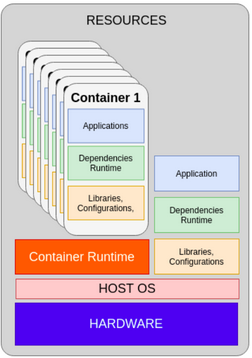
\includegraphics[width=0.3\textwidth]{04-figuras/containers.png}
    \caption[Estrutura do \emph{container} ]{Estrutura do \emph{container} (elaborada pelo autor)}
    \label{fig:container}
\end{figure}

\begin{figure}[!h]
    \centering
    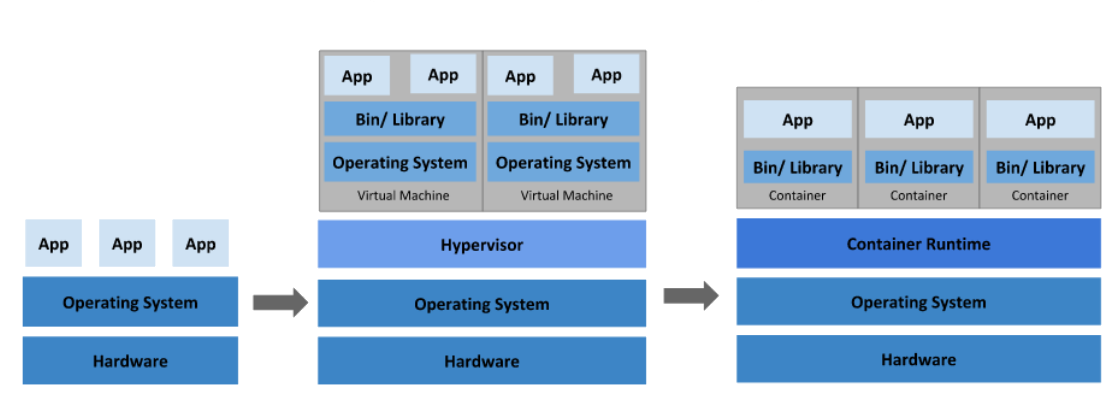
\includegraphics[width=0.8\textwidth]{04-figuras/vmsContainer.png}
    \caption[Eras de \emph{deployment}s e sua evolução por tecnologia base ]{Eras de \emph{deployment}s e sua evolução por tecnologia base (Fonte: The Linux Foundation\textregistered, 2021)}
    \label{fig:vmscontainer}
\end{figure}

Soluções como Apache Mesos, Hashicorp Nomad, e Docker Swarm também foram avaliadas pelo estudo de \cite{truyen_comprehensive_2021}, mas em todos os casos foram citadas diferenças significativas, especialmente no uso, sendo o Kubernetes\textregistered \ a melhor por eles avaliada. 

\section{Cluster orquestrador de \emph{container}}

Kubernetes\textregistered \ é a consolidação de quinze anos de trabalho da Google\textregistered \ com orquestração de cargas de trabalho, processamentos \emph{batch}, e um sistema interno de gerenciamento de \emph{cluster} orientado a \emph{container}s, o Borg \cite{verma_large-scale_2015}. 

As estruturas básicas do Kubernetes\textregistered \ são divididas em componentes com atribuições bem definidas, como na Figura \ref{fig:kubenode}. Os componentes que são essenciais à proposta deste trabalho são:
\begin{itemize}
    \item \emph{Kube-apiserver}, que concentra toda a api do kubernetes
    \item \emph{Kube-scheduler}, que avalia novos pods e em qual nó worker do \emph{cluster} eles serão alocados
    \item \emph{Kube-controller-manager}, que comporta os objetos de controle do kubernetes
    \item \emph{Kubelet}, responsável por repassar comando do control plane, para o worker e comunicar com \emph{container} \emph{runtime}
    \item \emph{Kube-proxy}, responsável por toda a estrutura de redes nativa do kubernetes e pods do \emph{cluster}
    \item \emph{Pod}, menor unidade de \emph{deployment}, podendo conter um conjunto de \emph{container}s que compõem uma solução.
\end{itemize}

\begin{figure}[!h]
    \centering
    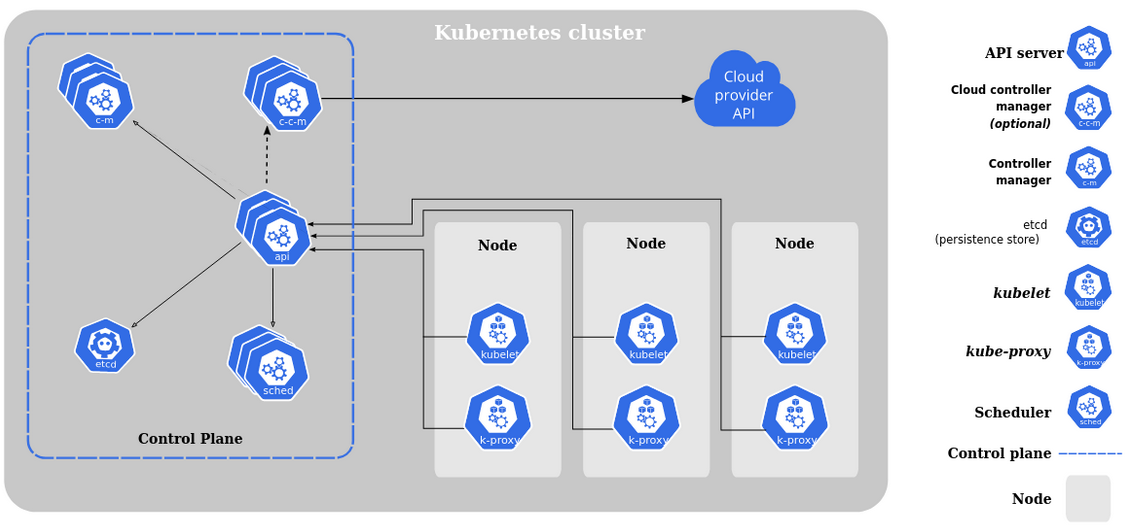
\includegraphics[width=0.8\textwidth]{04-figuras/kubeadm-node.png}
    \caption[Kubernetes arquitetura de componentes ]{Kubernetes arquitetura de componentes (Fonte: The Linux Foundation\textregistered, 2021)}
    \label{fig:kubenode}
\end{figure}



     % Fundamentação teórica
% -----------------------------------------------------------------------------
% Metodologia
% -----------------------------------------------------------------------------

\chapter{Metodologia}
\label{chap:metodologia}
\section{Disponibilidade dos recursos deste trabalho}
Todos os componentes definidos nesse trabalho estarão contidos em um ou mais repositórios públicos, garantindo assim a livre apreciação da comunidade não só científica, mas a todos os interessados na contribuição ou utilização sob a licença pública geral GNU versão 3 \cite{foss2022}.

\section{Especificação dos nós integrantes cluster de baixo custo}

A formação do cluster será de máquinas virtuais (VMs) e/ou físicas que possuem custo e capacidade computacionais mais baixos, com configurações comumente encontradas em computadores do tipo desktops, como os utilizados em residências, escritórios e laboratórios de informática genéricos.

A primeira versão dessa solução será realizada de maneira simulada, utilizando ambiente virtualizado com VMs que por sua vez serão provisionadas em hypervisors do tipo 2 \cite{comer_cloud_2021} (\emph{hosted hypervisor}), para garantir a simplicidade da implementação da primeira fase (TCC 1) e validar o conceito de provisionamento, configuração e \emph{deploy} de aplicações testes, bem como laboratório das ferramentas de monitoramento que serão utilizadas, a serem descritas a seguir. 

\begin{figure}[!h]
    \centering
    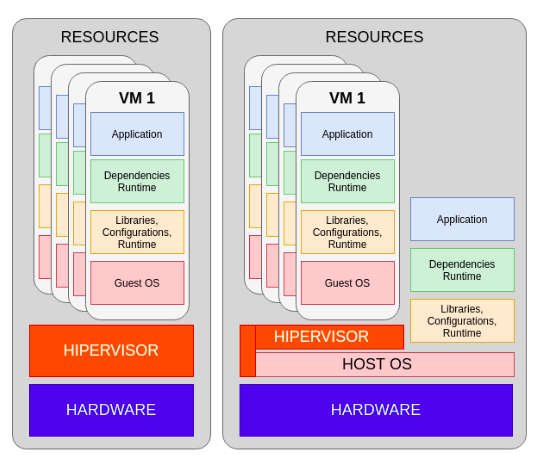
\includegraphics[width=0.8\textwidth]{04-figuras/vms.png}
    \caption{Hosted Hypervisor diagrama representativo de componentes (Fonte: Google Images, 2021)}
    \label{fig:vms}
\end{figure}

A versão final do projeto (ambas no TCC II) visa o provisionamento do cluster nos ambientes de teste configurados como descrito anteriormente, sendo que algumas premissas serão utilizadas, como o uso de mesmo sistema operacional e versão do mesmo em cada um desses computadores. Garantindo a redução de configuração necessária para a implementação. Outra premissa utilizada para esse estudo, será a utilização de uma rede comum aos computadores. 

O aproveitamento de computadores comuns já existentes e subutilizados seja por uso abaixo de sua capacidade ou ainda intervalos de ociosidade, qualifica o baixo custo da formação do cluster em questão, apresentando CAPEX (capital expenditure),  ou investimento inicial mínimo, se não zero, necessitando da interdisciplinaridade sugerida e defendida dentro das instituições para o qual esse trabalho intenta apresentar uma alternativa.

\section{Plataforma de orquestração de carga de trabalho}

A plataforma de cluster e orquestração de cargas de trabalho utilizadas nesse trabalho será o Kubernetes. A arquitetura de implementação do cluster será de multi-master com etcd \cite{etcd2022} (controlador de logs, e estado do cluster) atachado \cite{kubernetes2022}, ou rodando nos mesmo computadores masters do cluster. 
Essa arquitetura recomendada, garante a alta disponibilidade do cluster importante para que não haja interrupções inesperadas durante a orquestração das cargas de trabalho (execução, disponibilidade e garantia de estado desejado). Apenas não garantindo uma recuperação rápida de outages dos nós mestres, significando a perda de todos os estados e, com isso, havendo a necessidade de reconfiguração do cluster. Porém considerando os recursos limitados, na justificativa desse projeto, a alta disponibilidade de estado, significaria na obrigatoriedade do mesmo número de computadores disponibilizados para etcd e masters para controle dos estados.


\begin{figure}[!ht]
    \centering
    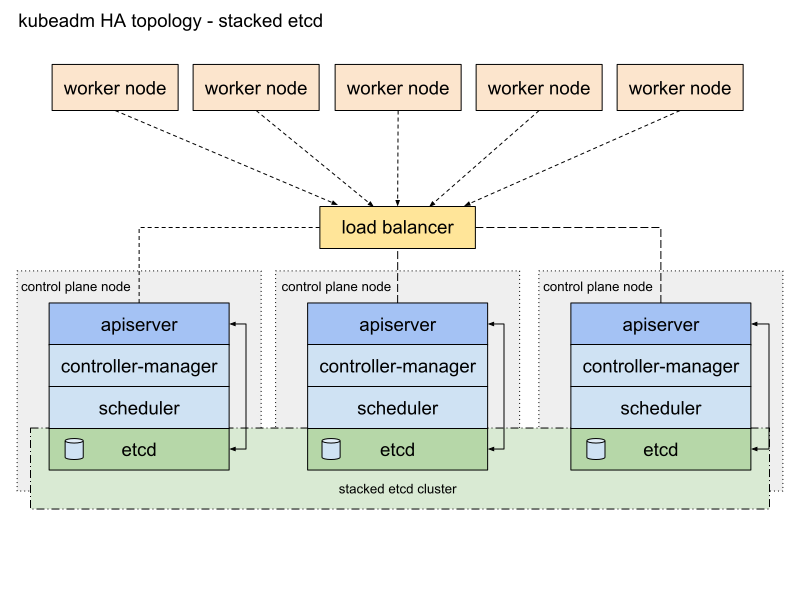
\includegraphics[width=0.8\textwidth]{04-figuras/kubeadm-ha-topology-stacked-etcd.png}
    \caption{Kubernetes Arquitetura de alta disponibilidade (Fonte: The Linux Foundation\textregistered, 2021)}
    \label{fig:kubeadmha}
\end{figure}


Toda a implementação da solução e os componentes relacionados serão conteinerizados, possibilitando  sua orquestração pelo cluster de Kubernetes\textregistered. Apenas as configurações dos clusters em si e seu provisionamento não estarão conteinerizados. Esses serão disponibilizados em outro repositório específico. 
Para ciclo de vida da aplicação e configurações gerais da solução será utilizado uma estratégia de organização de código em monorepo, facilitando a visualização, centralização, sincronização, padronização como benefícios primários e demonstrados na literatura reforçando a adoção dessa estratégia \cite{brito_monorepos_2018}.
\section{Configuração e provisionamento do cluster}
Para provisionamento do \emph{cluster} utilizaremos Ansible\textregistered da empresa RedHat\textregistered. Sua adoção se deu pela característica minimalista de configuração inicial, facilidade de uso e uma característica fundamental que diminui o \emph{overhead} de operação necessária para sua utilização, não possuir agente instalado nas no inventário de máquinas gerenciadas. 

O principal ganho em existente no uso de um sistema de gerenciamento de configuração (CMS) é o não gerenciamento do sistema para utilizá-lo, não há necessidade de configuração ou instalação de nenhum binário específico para sua utilização, reduzindo assim a complexidade de utilização inicial.

A configuração inicial é realizada pela disponibilidade de acesso via rede, python na máquina a ter sua configuração gerenciada (asset, ou recurso) e por meio de alguns tipos de autenticação (kerberos, WinRM, SSH etc), sendo no caso utilizado o protocolo SSH \cite{noauthor_rfc4254_nodate} por chaves assimétricas o que garante um nível aceitável de segurança, especialmente quando se é possível escolher os algoritmos de criptografia e suas possíveis variações como RSA e ED25519.

\section{Análise de dados}

O banco de dados “Vendas de Medicamentos Controlados e Antimicrobianos - Medicamentos Industrializados”, disponibilizado pelo governo brasileiro (via portal dados.gov.b), será utilizado nesse trabalho. Os anos correspondentes dos dados são no período entre 2014 e 2021 e o banco possui mais de 70 GB  e mais de 530 milhões de linhas, sendo assim suficiente para ser utilizado como carga de trabalho ao se calcular uma regressão linear para consumo do medicamento de azitromicina.
Como caso base para comparação e teste do modelo proposto, em termos de tempo para processamento da análise proposta acima,  utilizaremos um único computador (desktop) com capacidade equivalente a 8 computadores de menor capacidade (1vCPU e 2GB De RAM) designados com nós do cluster, portanto contendo recursos de  8 vCPUs e 16GB de RAM. 

\section{Monitoramento}

Serão utilizados para monitoramento de execução das cargas de trabalho Prometheus\textregistered  e para visualização dos dados Grafana\textregistered, ambos sendo configurados a partir do provisionamento do cluster, ainda com a ferramenta proposta inicialmente Ansible\textregistered. Dessa forma será possível avaliar parâmetros de taxa de lotação das máquinas base, pelo parâmetro de processador e memória, operações de leitura e escrita no disco e também tráfego de rede. Por meio dessas ferramentas será possível ainda, avaliar dados de tempo de execução de cargas de trabalho em ambos os ambientes propostos e assim poder compará-los sob eficiência de uso de hardware.

\section{Comparação entre tipos de virtualização}

A arquitetura do tipo x86 foi o tipo mais comum de arquitetura de computadores e boa parte da tecnologia de virtualização inicialmente foi desenvolvida nessa arquitetura (FAYYA, 2013). Nesse contexto será também utilizado na construção desse trabalho virtualizações com guest e host OS  em x86, para garantir que outros estudos possam ser relacionados na obtenção dos resultados desse trabalho.
Como descrito anteriormente, serão utilizadas maquinas virtuais com 2GB de RAM e containers com limitações de mesmo tamanho para a realização de configuração do cluster nesses ambientes, e a partir destes a execução dos workloads.

O tipo de teste de aplicação será um macrobenchmark (system level benchmark) \cite{huge2008,scheepers2014virtualization} comparando parâmetros de uso de CPU, memória e tempo de execução da carga de trabalho proposta na sessão 3.1.5 deste trabalho. Os parâmetros serão avaliados  tanto na máquina de suporte a virtualização e também nas máquinas virtuais e containers, bem como o tempo provisionamento do container da carga de trabalho, tempo de execução e quantidades de falhas.

Esse método USE (Usage, Saturation and Errors) \cite{greg2022} será utilizado para extrair e apresentar métricas e avaliar possíveis problemas, sendo que esse não é o foco do trabalho, mas captura de forma adequada os parâmetros de hardware citados acima.

Para controle de tempo será por meio de ferramentas de APM (Application Performance Management) associada a aplicação da carga de trabalho. Dessa forma garantimos a avaliação de qualidade e possíveis problemas, tempos de execução dentre outros possíveis problemas e métricas de performance da aplicação \cite{tang2021systematical}.


\section{Cronograma}
A primeira parte do Trabalho de Conclusão de Curso consiste em um estudo dos métodos de virtualização, plataformas elegidas como possíveis soluções e a composição de arquitetura da plataforma de orquestração das cargas de trabalho. Bem como a construção de um modelo inicial de assim como a definição de uma arquitetura de referência a ser refinada no TCC II junto aos demais diagramas do sistema. A solução proposta para realizar tanto a orquestração como também a comparação das cargas de trabalho também serão validadas durante a execução do TCC II.
Na \ref{fig:cronograma} é apresentado o cronograma total:

\begin{landscape}
\begin{figure}[!ht]
    \centering
    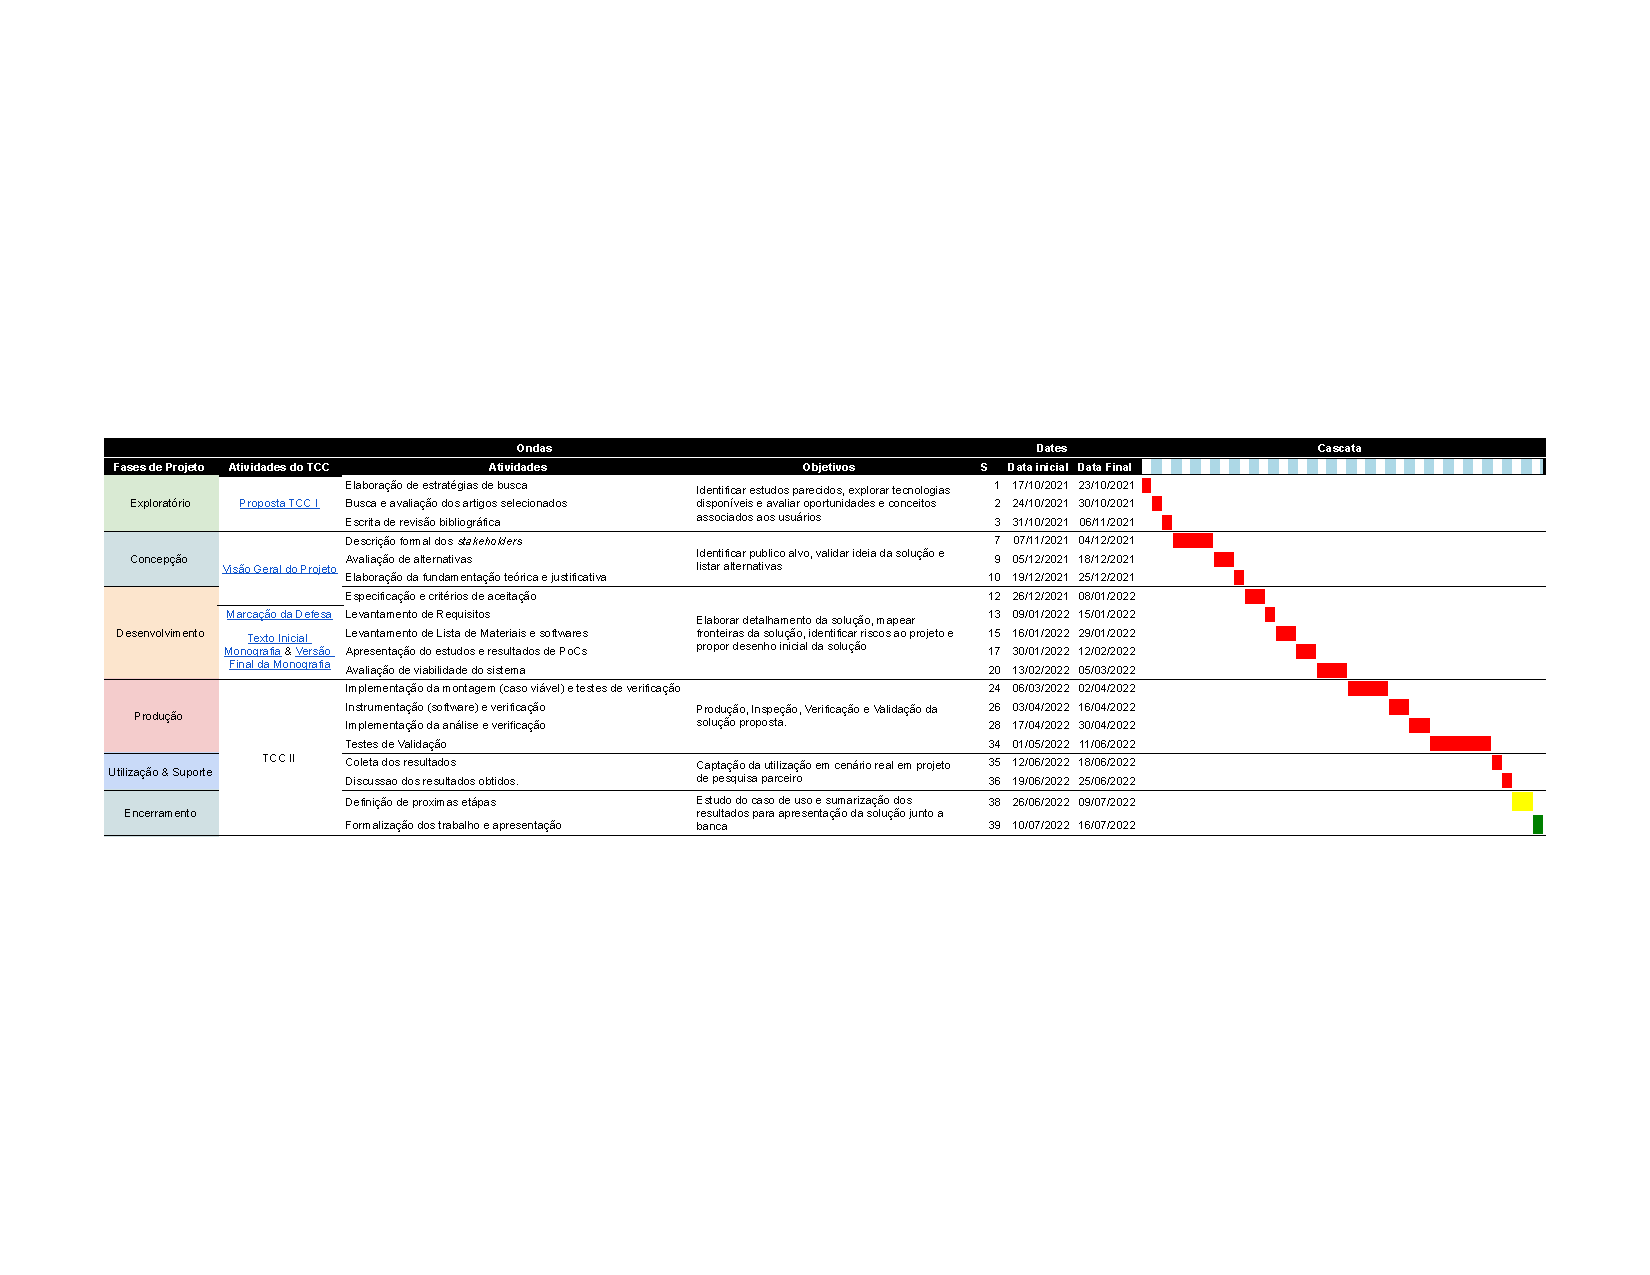
\includegraphics[width=\linewidth]{04-figuras/TCC cronograma - Sheet1.pdf}
    \caption{Cronograma geral do trabalho}
    \label{fig:cronograma}
\end{figure}
\end{landscape}               % Metodologia
% -----------------------------------------------------------------------------
% Resultados
% -----------------------------------------------------------------------------

\chapter{Análise e Discussão dos Resultados}

Cada capítulo deve conter uma pequena introdução (tipicamente, um ou dois parágrafos), em seção não numerada, que deve deixar claro o objetivo e o que será discutido no capítulo, bem como a organização do capítulo.

\section{Título da seção}
\label{sec:titSecResult}

Inserir seu texto aqui...
                % Resultados
% -----------------------------------------------------------------------------
% Conclusão
% -----------------------------------------------------------------------------

\chapter{Conclusão}
\label{chap:conclusao}

O desenvolvimento do presente trabalho possibilitou a avaliação de diferentes tipos de virtualização para comparação na implementação da plataforma de orquestração de cargas de trabalho de analise de dados em saúde. Através de profunda revisão bibliográfica foram identificados outras plataforma de orquestração de cargas de trabalhos e foi possível fazer uma avaliação critica baseada nos requisitos disponibilizados nas documentações oficiais, bem como a avaliação crítica do proposito ao qual o presente trabalho se propunha. Ainda na literatura, foi possível encontrar dados e informações a respeito dos impactos socio-econômicos resultantes da restrição orçamentária a pesquisa de uma forma geral. Em específico no caso desse trabalho para análise de dados em saúde, especialmente no auxilio de extração de informações relevantes de grande base de dados. O que torna possível a tomada de decisão em saúde pautada em dados e também auxilia a população a ter melhor noção, baseada em dados, da situação de saúde no qual se encontra e assim poder auditar os órgãos públicos responsáveis pela condução do SUS e políticas de saúde associadas.

\section{Trabalhos Futuros}
\label{sec:trabalhosFuturos}

Na continuação deste trabalho, o provisionamento do ambiente de testes com as devidas restrições e sua consequente avaliação será realizada, coletando dados de tempo de execução, taxa de utilização de memória e CPU, para comparação das duas propostas de sistemas virtualizados. Permitindo assim avaliar qual estratégia mais adequada para simulação de implementação e orquestração de dados.
No encerramento desse trabalho possibilita-se que o conhecimento desenvolvido ao longo do TCC possibilite a avaliação de implementação em maquinas físicas, podendo levar ao recrutamento de maquinas heterogêneas e de diversas configurações de hardware afim de criar um ou mais \emph{clusters} com capacidade suficiente para escalonar diversos tipos de cargas de trabalho, a exemplo da desse trabalho afim de possibilitar o processamento de dados massivos.

% \section{Considerações Finais}
% \label{sec:consideracoesFinais}

% As derradeiras palavras para encerramento do seu trabalho acadêmico.

% -----------------------------------------------------------------------------
% Observação: A norma ABNT estabelece que em qualquer tipo de trabalho
% acadêmico monográfico deve haver um capítulo de conclusão
% -----------------------------------------------------------------------------
                 % Conclusão

% Insere os elementos pós-textuais
\postextual
% -----------------------------------------------------------------------------
% Referências
% -----------------------------------------------------------------------------

% -----------------------------------------------------------------------------
% Carrega o arquivo "base-referencias.bib" e extrai automaticamente as referências citadas
% -----------------------------------------------------------------------------

\bibliography{./referencias}{}
\bibliographystyle{abntex2-alf} % Define o estilo ABNT para formatar a lista de referências

% -----------------------------------------------------------------------------
% Este arquivo não necessita de ser editado.
% -----------------------------------------------------------------------------
           % Referências
% % -----------------------------------------------------------------------------
% Apêndices
% -----------------------------------------------------------------------------

\begin{apendicesenv}
\partapendices

% -----------------------------------------------------------------------------
% Primeiro apêndice
% -----------------------------------------------------------------------------

\chapter{Nome do apêndice} % Edite para alterar o título deste apêndice
\label{chap:apendiceA}

Lembre-se que a diferença entre apêndice e anexo diz respeito à autoria do texto e/ou material ali colocado.

Caso o material ou texto suplementar ou complementar seja de sua autoria, então ele deverá ser colocado como um apêndice. Porém, caso a autoria seja de terceiros, então o material ou texto deverá ser colocado como anexo.

Caso seja conveniente, podem ser criados outros apêndices para o seu trabalho acadêmico. Basta recortar e colar este trecho neste mesmo documento. Lembre-se de alterar o "label"{} do apêndice.

Não queira colocar tudo que é complementar em um único apêndice. Organize seus apêndices de modo a que, em cada um deles, haja um único tipo de conteúdo. Isso facilita a leitura e compreensão para o leitor do trabalho. É para ele que você escreve.

% -----------------------------------------------------------------------------
% Novo apêndice
% -----------------------------------------------------------------------------

\chapter{Estrutura de trabalhos acadêmicos}
\label{chap:apEstrTrabAcad}

Quanto à estrutura do trabalho acadêmico, esta varia sobremaneira, a depender da conveniência do autor e seu(s) respectivo(s) orientador(es). No entanto, de acordo com as normas ABNT, alguns elementos são obrigatórios.

A título de sugestão, e apenas isso, a \autoref{fig:estrutura-projeto-qualificacao} apresenta uma estrutura para um projeto de qualificação de mestrado ou doutorado, conforme a norma \citeonline{NBR14724:2011}.

\begin{figure}[!htb]
    \centering
    \caption{Estrutura sugerida de um Projeto de Qualificação para os cursos de Mestrado ou Doutorado}
    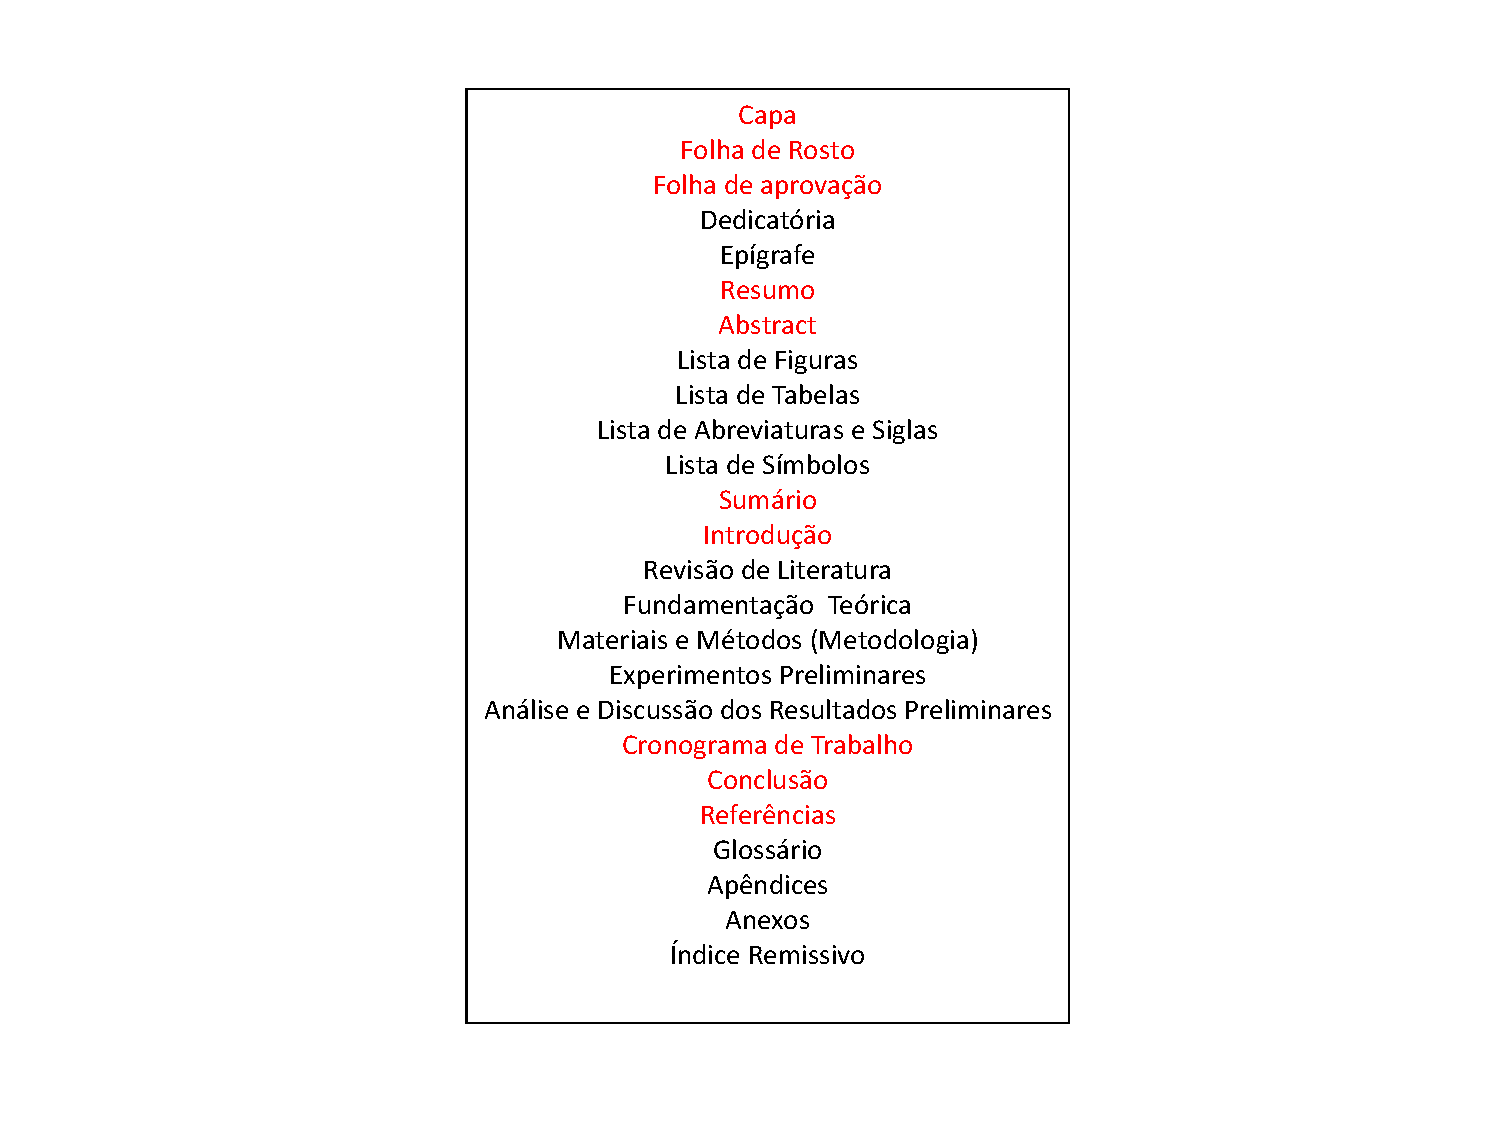
\includegraphics[width=0.5\textwidth]{./04-figuras/estrutura-projeto-qualificacao}
    \label{fig:estrutura-projeto-qualificacao}
\end{figure}

Já a \autoref{fig:estrutura-tese-dissertacao} apresenta uma estrutura para uma tese de doutorado ou dissertação de mestrado, conforme a norma \citeonline{NBR14724:2011}.

Cabe ressaltar que, em todas as figuras, os elementos obrigatórios estão destacados em vermelho, os demais são opcionais.

\begin{figure}[!htb]
    \centering
    \caption{Estrutura sugerida de uma Tese de Doutorado ou Dissertação de Mestrado}
    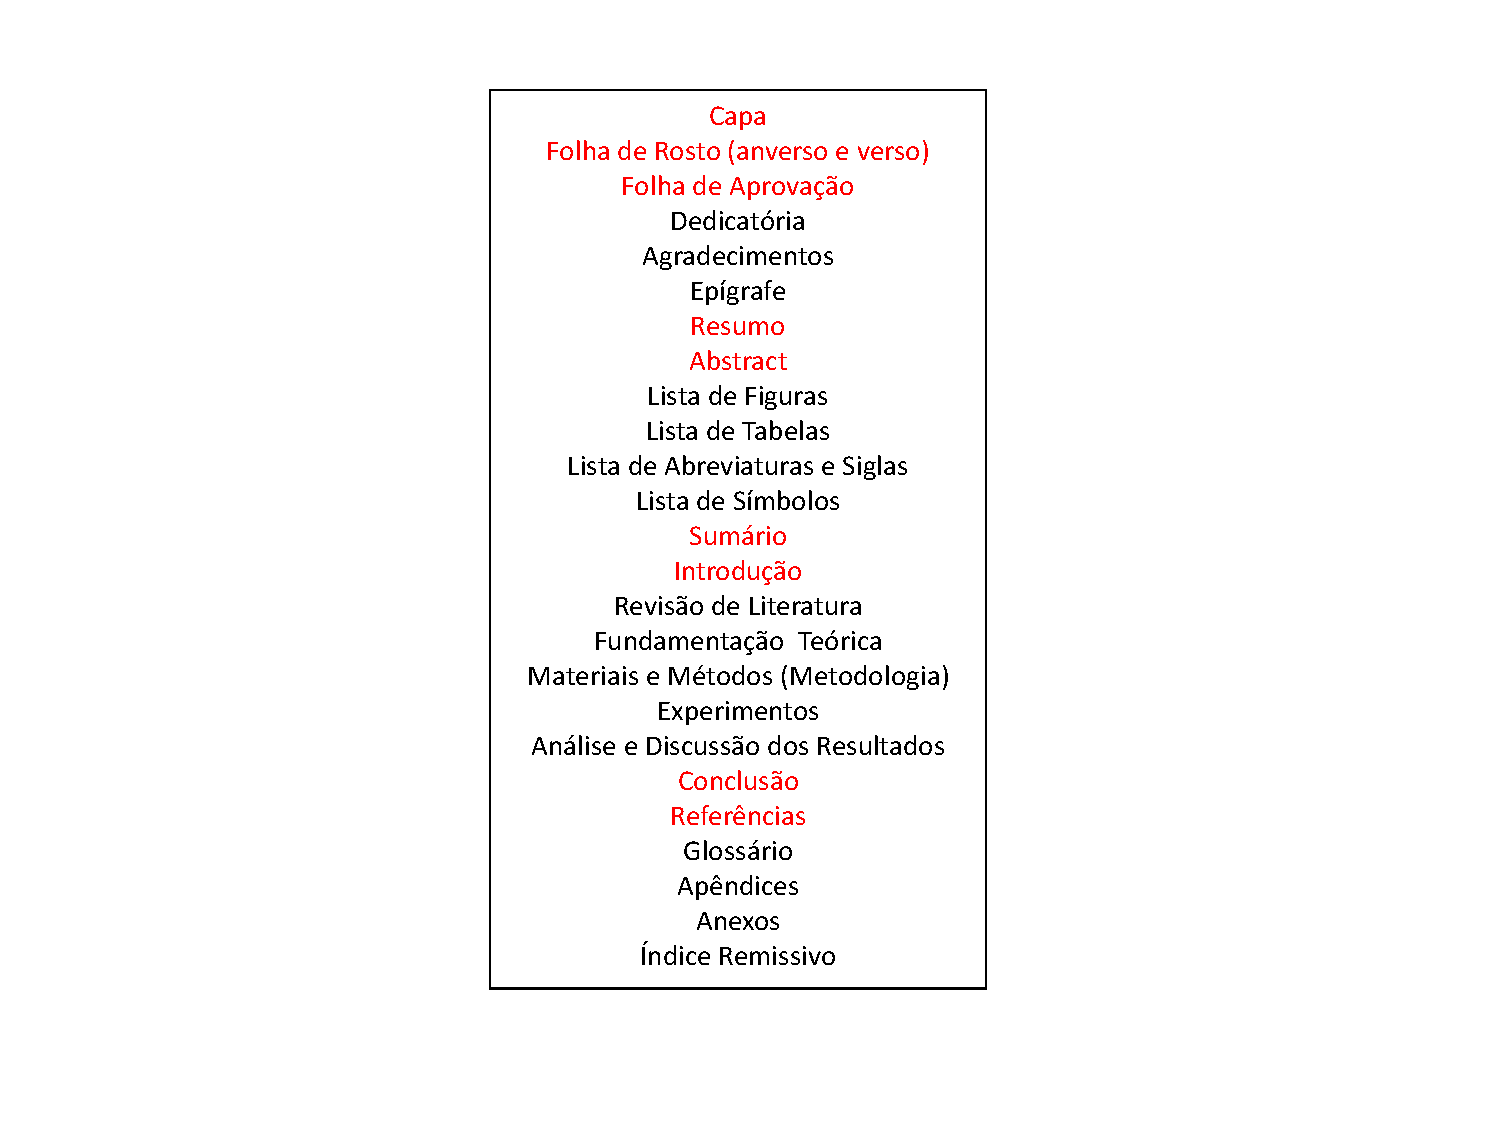
\includegraphics[width=0.5\textwidth]{./04-figuras/estrutura-tese-dissertacao}
    \label{fig:estrutura-tese-dissertacao}
\end{figure}

Observe que a estrutura de um projeto de qualificação é muito similar à da tese ou dissertação. A única diferença existente é que num projeto de qualificação o autor certamente terá, via de regra, apenas resultados parciais e preliminares. Além disso, estando o trabalho ainda em andamento, há que se apresentar um cronograma de trabalho que evidencie que o mesmo poderá ser concluído dentro dos prazos estabelecidos pelo programa.

Por fim, como foi dito, este  \emph{template} pode ser utilizado para outros trabalhos acadêmicos. Neste caso, a \autoref{fig:estrutura-projeto-pesquisa} apresenta uma sugestão de projeto de pesquisa a ser submetido ao programa para fins de admissão ao mesmo, conforme a norma \citeonline{NBR15287:2005}.

\begin{figure}[!htb]
    \centering
    \caption{Estrutura sugerida de um projeto de pesquisa para admissão ao PPGMMC}
    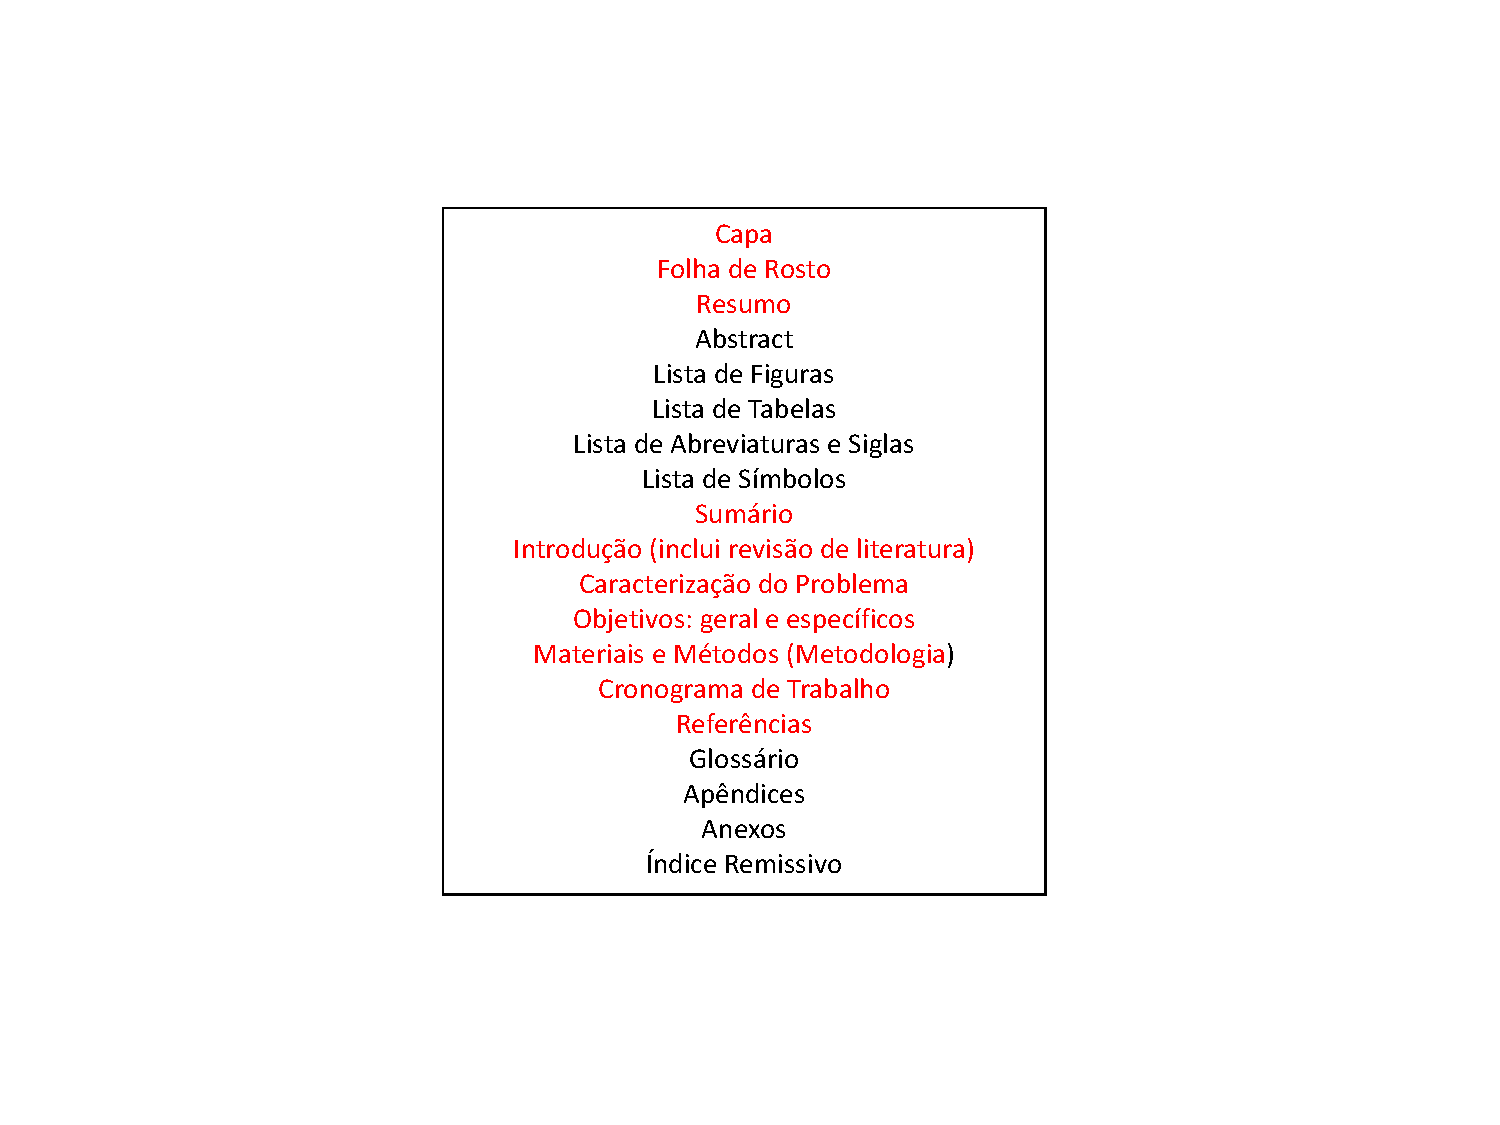
\includegraphics[width=0.6\textwidth]{./04-figuras/estrutura-projeto-pesquisa}
    \label{fig:estrutura-projeto-pesquisa}
\end{figure}

Você deverá editar o arquivo principal {\ttfamily meuTrabalhoAcademico.tex} para fazer os ajustes necessários, reiterando que as estruturas apresentadas são mera sugestão.

A inclusão de reticências (\ldots) no texto deverá ser feita através de um comando especial denominado \verb|\ldots| \cite{LaTeX2014}. Assim esse comando deverá ser utilizado ao invés da digitação de três pontos.

Para melhor entendimento do uso do estilo de formatação, aconselha-se que o potencial usuário análise os comandos existentes no arquivo {\ttfamily main.tex} e os resultados obtidos no arquivo {\ttfamily main.pdf} depois do processamento pelo software \LaTeX{} + \textsc{Bib}\TeX{} \cite{LaTeX2014,BibTeX2014}.
Recomenda-se a consulta ao material de referência do software para a sua correta utilização \cite{Lamport1986,Buerger1989,Kopka2003,Mittelbach2004}.

Finalmente, este modelo apresenta um arquivo {\ttfamily makefile} para agilizar a compilação do documento \LaTeX{} e do \textsc{Bib}\TeX{}. portanto, para gerar o documento final no formato PDF, basta apenas executar o comando {\ttfamily make all} no linux. Para limpar os arquivos temporários, basta digitar o comando {\ttfamily make clean}.

O estilo de documento utilizado é o {\ttfamily abntex2}.
Através desse estilo a constituição do documento torna-se facilitada, uma vez que o mesmo possui comandos especiais para auxiliar a distribuição/definição das diversas partes constituintes do projeto.
Esse estilo é baseado nas normas da ABNT\index{ABNT}.

Maiores detalhes relacionados aos comandos existentes no estilo poderão ser adquiridos através da documentação disponível no site \href{https://code.google.com/p/abntex2/}{https://code.google.com/p/abntex2/} \cite{abnTeX22014b}.

Uma das principais vantagens do uso do estilo de formatação para \LaTeX{}  é a formatação \textit{automática} dos elementos que compõem um documento acadêmico, tais como capa, folha de rosto, dedicatória, agradecimentos, epígrafe, resumo, abstract, listas de figuras, tabelas, siglas e símbolos, sumário, capítulos, referências, etc.

% -----------------------------------------------------------------------------
% Novo apêndice
% -----------------------------------------------------------------------------

\chapter{Sobre as ilustrações}
\label{chap:apSobreIlust}

A seguir ilustra-se a forma de incluir ilustrações no corpo do texto. Pela norma figuras, tabelas, quadros, equações, quadros, algoritmos, diagrama, etc. são tipos específicos de ilustrações. As ilustrações (pelo menos alguns tipos específicos) serão indexadas automática em suas respectivas listas.

A numeração sequencial de figuras, tabelas e equações ocorre de modo automático.

Referências cruzadas são obtidas através dos comandos \verb|\label{}| e \verb|\ref{}|. Por exemplo, não é necessário saber que o número de certo capítulo é \ref{chap:fundamentacaoTeorica} para colocar o seu número no texto. Alternativamente se pode usar desta forma: \autoref{chap:fundamentacaoTeorica}. Isto facilita muito a inserção, remoção ou relocação de elementos numerados no texto (fato corriqueiro na escrita e correção de um documento acadêmico) sem a necessidade de renumerá-los todos.

\section{Figuras}
\label{sec:figuras}

Abaixo é apresentado um exemplo de figura.

A \autoref{fig:kdtree} aparece automaticamente na lista de figuras.

Para uso avançado de imagens no \LaTeX{}, recomenda-se a consulta de literatura especializada \cite{Goossens2007}.

\begin{figure}[!htb]
    \centering
    \caption{Exemplo da estrutura de uma árvore KD}
    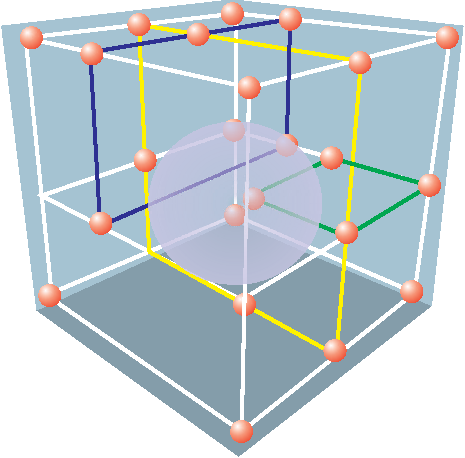
\includegraphics[width=0.5\textwidth]{./04-figuras/figura-exemplo}
    \fonte{\citeonline{Souza2012}}
    \label{fig:kdtree}
\end{figure}

\section{Quadros e tabelas}
\label{sec:tabelas}

Também é apresentado o exemplo do \autoref{qua:comparabd} e da \autoref{tab:testes}, que aparece automaticamente na lista de quadros e tabelas.

Informações sobre a construção de tabelas no \LaTeX{} podem ser encontradas na literatura especializada \cite{Lamport1986,Buerger1989,Kopka2003,Mittelbach2004}.

\begin{quadro}[!htb]
    \centering
    \caption{Hierarquia de restrições das questões.\label{qua:comparabd}}
    \begin{tabular}{|p{7cm}|p{7cm}|}
        \hline
        \textbf{BD Relacionais} & \textbf{BD Orientados a Objetos} \\
        \hline
        Os dados são passivos, ou seja, certas operações limitadas podem ser automaticamente acionadas quando os dados são usados. Os dados são ativos, ou seja, as solicitações fazem com que os objetos executem seus métodos. & Os processos que usam dados mudam constantemente. \\
        \hline
    \end{tabular}
    \fonte{\citeonline{Carvalho2001}}
\end{quadro}


Muitos confundem, mas existem diferenças entre tabelas e quadros.

Um quadro é formado por linhas horizontais e verticais, sendo, portanto ``fechado''. Você deverá utilizar um quadro quando o conteúdo é majoritariamente não-numérico. O número do quadro e o título vem acima do quadro, e a fonte, deve vir abaixo.

Uma tabela é formada apenas por linhas verticais, sendo, portanto ``aberta''. Você deverá utilizar uma tabela quando o conteúdo é majoritariamente numérico. O número da tabela e o título vem acima da tabela, e a fonte, deve vir abaixo, tal como no quadro.

Exemplo de tabela:

\begin{table}[!htb]
    \centering
    \caption[Resultado dos testes]{Resultado dos testes.
    \label{tab:testes}}
    \begin{tabular}{rrrrr}
        \toprule
            & Valores 1 & Valores 2 & Valores 3 & Valores 4 \\
        \midrule
            Caso 1 & 0,86 & 0,77 & 0,81 & 163 \\
            Caso 2 & 0,19 & 0,74 & 0,25 & 180 \\
            Caso 3 & 1,00 & 1,00 & 1,00 & 170 \\
        \bottomrule
    \end{tabular}
\end{table}


\section{Equações}
\label{sec:equacoes}

A transformada de Laplace é dada na \autoref{eq:laplace}, enquanto a Eq. \ref{eq:dft} apresenta a formulação da transformada discreta de Fourier bidimensional\footnote{Deve-se reparar na formatação esteticamente perfeita destas equações.}. Observe que utilizamos propositalmente duas formas distintas para referenciar as equações.

\begin{equation}
    X(s) = \int\limits_{t = -\infty}^{\infty} x(t) \, \text{e}^{-st} \, dt
    \label{eq:laplace}
\end{equation}

\begin{equation}
    F(u, v) = \sum_{m = 0}^{M - 1} \sum_{n = 0}^{N - 1} f(m, n) \exp \left[ -j 2 \pi \left( \frac{u m}{M} + \frac{v n}{N} \right) \right]
    \label{eq:dft}
\end{equation}

\section{Algoritmos}\label{sec:algoritmos}

Os algoritmos devem ser feitos segundo o modelo abaixo. Para isso, utilizar o pacote {\ttfamily algorithm2e} no início do arquivo principal como neste exemplo.
\\
\\

\begin{algorithm}
    \caption{Algoritmo para remoção aleatória de vértices}
    \KwIn{o número $n$ de vértices a remover, grafo original $G(V, E)$}
    \KwOut{grafo reduzido $G'(V,E)$}
    $removidos \leftarrow 0$ \\
    \While {removidos $<$ n } {
        $v \leftarrow$ Random$(1, ..., k) \in V$ \\
            \For {$u \in adjacentes(v)$} {
                remove aresta (u, v)\\
                $removidos \leftarrow removidos + 1$\\
            }
            \If {há  componentes desconectados} {
                remove os componentes desconectados\\
            }
        }
\end{algorithm}


% -----------------------------------------------------------------------------
% Novo apêndice
% -----------------------------------------------------------------------------

\chapter{Sobre as listas}
\label{chap:apSobreLista}

Para construir listas de "\textit{bullets}"{} ou listas enumeradas, inclusive listas aninhadas, é utilizado o pacote \verb|paralist|.

O exemplo a seguir ilustra duas listas não numeradas aninhadas, utilizando o ambiente \verb|\itemize|. Observe a indentação, bem como a mudança automática do tipo de "\textit{bullet}"{} nas listas aninhadas.

\begin{itemize}
    \item item não numerado 1
    \item item não numerado 2
    \begin{itemize}
        \item subitem não numerado 1
        \item subitem não numerado 2
        \item subitem não numerado 3
    \end{itemize}
    \item item não numerado 3
\end{itemize}

Por outro lado, o exemplo a seguir ilustra duas listas numeradas aninhadas, utilizando o ambiente \verb|\enumerate|. Observe a numeração progressiva e indentação das listas aninhadas.

\begin{enumerate}
    \item item numerado 1
    \item item numerado 2
    \begin{enumerate}
        \item subitem numerado 1
        \item subitem numerado 2
        \item subitem numerado 3
    \end{enumerate}
    \item item numerado 3
\end{enumerate}

Cabe ressaltar que os ambientes \verb|\itemize| e \verb|\enumerate| podem ser utilizados alternativamente. No entanto, durante a compilação pdflatex são apresentados erros associados a estes ambientes, porém o pdf é gerado corretamente. Trata-se de um "\textit{bug}"{} que ainda não conseguimos resolver. Caso conheça a solução, por favor, comunique-nos para que possamos incluí-la numa futura atualização deste modelo.

% -----------------------------------------------------------------------------
% Novo apêndice
% -----------------------------------------------------------------------------

\chapter{Sobre citações e chamadas de referências}
\label{chap:apSobreCita}

Citações são trechos transcritos ou informações retiradas das publicações consultadas para a realização do trabalho.
As citações são utilizadas no texto com o propósito de esclarecer, completar, embasar ou corroborar as ideias do autor.

Todas as publicações consultadas e efetivamente utilizadas (por meio de citações) devem ser listadas, obrigatoriamente, nas referências bibliográficas, de forma a preservar os direitos autorais e intelectuais.

A norma ABNT NBR:10520-2002 classifica as citações em: citações livres e citações literais.

\section{Citações livres}
\label{sec:citacoesLivres}

Nas citações livres, reproduzem-se as ideias e informações de um autor, sem, entretanto, ``copiar letra por letra'' o texto do autor. Sendo assim, não há muito a dizer sobre como fazer citações livres, exceto que há que se tomar o devido cuidado com o "recortar e colar e modificar"{} para que não se caracterize plágio.

Quanto à chamada da referência, ela pode ser feita de duas maneiras distintas, conforme o nome do(s) autor(es) façam parte do seu texto ou não. Os exemplos a seguir ilustram estas duas possibilidades.

Enquanto \citeonline{Maturana2003} defendem uma epistemologia baseada na biologia. Para os autores, é necessário rever \ldots.

Por outro lado, \citeonline{Barbosa2004} contra-argumenta afirmando que \ldots.

Acima, as chamadas de referências foram feitas com o comando \verb|\citeonline{chave}|, que produzirá a formatação correta, conforme a norma ABNT.

Observe que em ambos os casos anteriores, a frase fica incompleta e incompreensível caso as palavras "Maturana e Varela"{} e "Barbosa et al."{} não sejam "pronunciadas"{}. Ou seja, os nomes dos autores fazem parte da frase. Neste caso, a formatação automática da chamada de referência coloca os nomes dos autores seguido, entre parêntesis pelo ano de publicação da obra referenciada. Isso apenas no caso em que se usa o esquema autor-ano, que é \textit{padrão} neste modelo \LaTeX{}.

A segunda maneira de fazer uma chamada de referência deve ser utilizada quando se quer evitar uma interrupção na sequência do texto, o que poderia, eventualmente, prejudicar a leitura.

Assim, a citação livre é feita e imediatamente após a obra referenciada deve ser colocada entre parênteses. Porém, neste caso específico, o nome do autor deve vir em caixa alta, seguido do ano da publicação, como nos exemplos a seguir.

Há defensores da epistemologia baseada na biologia que argumentam em favor da necessidade de \ldots \cite{Maturana2003}.

Por outro lado, há os que contra-argumentam afirmando que \ldots  \cite{Barbosa2004}.

Nos dois casos imediatamente acima a chamada de referência deve ser feita com o comando \verb|\cite{chave}|, que produzirá a formatação correta, conforme a norma ABNT.

Observe que o estilo de redação das frases teve que ser modificado para torná-las compreensíveis sem a menção explícita dos nomes dos autores. Estes agora não são parte integrante da frase, ficam entre parêntesis. Neste caso, a formatação automática da chamada de referência coloca, entre parêntesis, os nomes dos autores seguido pelo ano de publicação da obra referenciada. Novamente, apenas no caso em que se usa o esquema autor-ano, que é \textit{padrão} neste modelo \LaTeX{}.

Por fim, cabe chamar a atenção para o detalhe do termo \textit{et al.} que deve ser utilizado quando o trabalho citado possui mais de três autores. Esse recurso é automatizado pelo estilo {\ttfamily abntex2}. Caso não haja desejo em abreviar o nome dos demais autores através do termo \textit{et al.}, deve-se incluir a opção {\ttfamily abnt-no-etal-label}.

\section{Citações literais}
\label{sec:citacoesLiterais}

Nas citações literais, reproduzem-se as ideias e informações de um autor, exatamente como este a expressou, ou seja, faz-se uma ``cópia letra por letra'' do texto do autor. Sendo assim, obviamente, a obra citada deve ser referenciada, sob pena de se caracterizar plágio.

Quanto à chamada da referência, ela pode ser feita de qualquer das duas maneiras mencionadas na \autoref{sec:citacoesLivres}, conforme o nome do(s) autor(es) façam parte do seu texto ou não.

Há duas maneiras distintas de se fazer uma citação literal, conforme o trecho citado seja longo ou curto.

Quando o trecho citado é longo (4 ou mais linhas) deve-se usar um parágrafo específico para a citação, na forma de um texto recuado (4 cm da margem esquerda), com tamanho de letra menor do aquela utilizada no texto e espaçamento entrelinhas simples. Veja o exemplo abaixo.

\begin{citacao}
    Desse modo, opera-se uma ruptura decisiva entre a reflexividade filosófica, isto é a possibilidade do sujeito de pensar e de refletir, e a objetividade científica.     Encontramo-nos num ponto em que o conhecimento científico está sem consciência. Sem consciência moral, sem consciência reflexiva e também subjetiva. Cada vez mais o desenvolvimento extraordinário do conhecimento científico vai tornar menos praticável a própria possibilidade de reflexão do sujeito sobre a sua pesquisa \cite[p.~28]{Silva2000}.
\end{citacao}

Para se criar o efeito demonstrado na citação anterior, deve-se utilizar o comando:

\begin{verbatim}
\begin{citacao}
<citacao>
\end{citacao}
\end{verbatim}

Acima, para a chamada da referência o comando \verb|\cite[p.~28]{Silva2000}| foi utilizado, visto que os nomes dos autores não são parte do trecho citado.

Observe ainda que foi indicado o número da página da obra citada que contém o trecho citado. A localização precisa do trecho citado deve ser indicada sempre, exceto para artigos científicos (tipicamente com poucas páginas, o que geralmente não é o caso de artigos de revisão de literatura) e outros documentos com "poucas"{} páginas.

Alternativamente, é possível construir uma frase que contenha os autores, e irá encaminhar (por assim dizer) a citação literal. Assim sendo, note que pode após a citação literal não mais aparece o nome dos autores, visto que já se encontra no texto. Veja o exemplo seguinte.

No entanto, \citeonline[p.~33]{Silva2000}, ao fazerem as suas críticas à ciência moderna, afirmam:

\begin{citacao}
    Mas o curioso é que o conhecimento científico que descobriu os meios realmente extraordinários para, por exemplo, ver aquilo que se passa no nosso sol, para tentar conceber a estrutura das estrelas extremamente distantes, e até mesmo para tentar pesar o universo, o que é algo de extrema utilidade, o conhecimento científico que multiplicou seus meios de observação e de concepção do universo, dos objetos, está completamente cego, se quiser considerar-se apenas a si próprio!
\end{citacao}

Já quando o trecho citado é curto (3 ou menos linhas) ele deve inserido diretamente no texto entre aspas. Veja os dois exemplos seguintes, cada qual utilizando uma forma de chamada de referência.

A epistemologia baseada na biologia parte do princípio de que ``assumo que não posso fazer referência a entidades independentes de mim para construir meu explicar'' \cite[p.~35]{Maturana2003}.

A epistemologia baseada na biologia de \citeonline[p.~35]{Maturana2003} parte do princípio de que ``assumo que não posso fazer referência a entidades independentes de mim para construir meu explicar''.

Finalmente, e isto vale para citações curtas ou longas, caso seja necessário inserir ou suprimir (modificar de modo geral) qualquer palavra ou frase no trecho citado literalmente, qualquer que seja a finalidade, isto deve ser feito colocando sua intervenção entre colchetes retos e deve ser indicado explicitamente ao final da citação. Veja o exemplo seguinte.

A epistemologia baseada na biologia parte do princípio de que ``assumo que não posso fazer referencia [\textit{sic}] a \underline{entidades independentes} de mim [realidade objetiva] para construir meu explicar'' \cite[p.~35, comentários e grifo nosso]{Maturana2003}.

\section{Mais detalhes sobre as chamadas de referências}
\label{sec:referUtilizadas}

A seguir há mais exemplos dos comandos para as chamadas de referências e o resultado produzido.

\citeonline{Maturana2003} \ \ \  \verb|\citeonline{Maturana2003}|\\
\citeonline{Barbosa2004} \ \ \   \verb|\citeonline{Barbosa2004}|\\
\cite[p.~28]{Silva2000} \ \ \  \verb|\cite[p.~28]{Silva2000}|\\
\citeonline[p.~33]{Silva2000} \ \ \   \verb|\citeonline[p.~33]{v}|\\
\cite[p.~35]{Maturana2003} \ \ \   \verb|\cite[p.~35]{Maturana2003}|\\
\citeonline[p.~35]{Maturana2003} \ \ \   \verb|\citeonline[p.~35]{Maturana2003}|\\
\cite{Barbosa2004,Maturana2003} \ \ \   \verb|\cite{Barbosa2004,Maturana2003}|\\

Há que se tomar bastante cuidado com referências cujos autores têm nomes compostos, tipo João de Souza Júnior ou Antônio José da Silva Filho. Para que a formatação seja correta, os nomes dos autores no arquivo {\ttfamily .bib} deverá ser cadastrado de uma forma específica. Para maiores detalhes, veja o \autopageref{chap:anexoB} \footnote{O texto do anexo é de inteira responsabilidade do autor devidamente referenciado.}.

Os exemplos abaixo ilustram a formatação correta.

\cite[p.~28]{vanGELDER1998} \ \ \ \ \  \verb|\cite[p.~28]{vanGELDER1998}|\\
\citeonline[p.~28]{vanGELDER1998} \ \ \ \ \  \verb|\citeonline[p.~28]{vanGELDER1998}|\\

Observe que, a despeito do que está dito no \autoref{chap:anexoB}, ainda há falhas na formatação ABNT de nomes tipo \verb|van Gelder| quando utilizados em chamadas de referências que fazem parte do texto (\textit{e.g.}, \verb|\citeonline{vanGELDER1998}| que deveria produzir \verb|van Gelder (1998)|). Este problema pode ser contornado facilmente, simplesmente evitando o uso dessa forma de chamada de referência, preferindo sempre nestes casos, o uso da forma \textit{e.g.}, \verb|\cite{vanGELDER1998}| que será formatada corretamente, produzindo \verb|(van GELDER, 1998)|.

Observe ainda o caso em que é feita duas citações juntas \cite{Santos2003, Neubert2001} e como citar endereços Web \cite{IRL2014}.

% -----------------------------------------------------------------------------
% Novo apêndice
% -----------------------------------------------------------------------------

\chapter{Sobre as referências bibliográficas}
\label{chap:apSobreRefer}

A bibliografia é feita no padrão \textsc{Bib}\TeX{}. As referências são colocadas em um arquivo separado. Os elementos de cada item bibliográfico que devem constar nas referências bibliográficas são apresentados a seguir. Tais referências bibliográficas devem seguir a norma \citeonline{NBR6023:2002} da ABNT\footnote{As normas técnicas da ABNT não são gratuitas.}.

\section{Entradas de referências}
\label{sec:entradasRefs}

Entradas são objetos de citação bibliográficas. Dito de outra forma, são as categorias dos tipos de documentos e materiais componentes da bibliografia. A classe abn\TeX{} define as seguintes entradas:

\begin{verbatim}
@book
@inbook
@article
@phdthesis
@mastersthesis
@monography
@techreport
@manual
@proceedings
@inproceedings
@journalpart
@booklet
@patent
@unpublished
@misc
\end{verbatim}

Cada entrada é formatada pelo pacote \citeonline{abnTeX22014d} de uma forma específica. Algumas entradas foram introduzidas especificamente para atender à norma \citeonline{NBR6023:2002}, são elas: \verb|@monography|, \verb|@journalpart|,\verb|@patent|. As demais entradas são padrão \textsc{Bib}\TeX{}. Para maiores detalhes, refira-se a \citeonline{abnTeX22014d}, \citeonline{abnTeX22014b}, \citeonline{abnTeX22014c}.

A entrada \verb|@monography| é utilizada para cadastrar referências a trabalhos de conclusão de curso, monografias de cursos de especialização (pós-graduação \textit{lato sensu}), e outros trabalhos monográficos, exceto dissertação de mestrado e tese de doutorado. Eu particularmente, não considero que a formatação deste tipo de entrada está adequado. Para um trabalho de conclusão de curso (TCC) de curso de graduação, que deveria ser formatado como "[\ldots] Trabalho de Conclusão de Curso (Bacharelado em Engenharia de Computação) [\ldots]"{}; no entanto o uso de \verb|@monography| irá produzir "[\ldots] Monografia (Bacharelado em Engenharia de Computação) [\ldots]"{}. A própria  \citeonline{NBR6023:2002}, na seção 8.11.4, apresenta um exemplo com a formatação diferente daquela proporcionada por \citeonline{abnTeX22014d}.

A entrada \verb|@journalpart| é utilizada, conforme diz o manual \cite{abnTeX22014d}, para cadastrar referências e formatar partes de periódicos. Não fica claro o que se quer dizer com partes de journal. Em alguns casos, tais partes são artigos - e portanto, deveriam ser registradas como \verb|@article| - noutros casos, parece serem matérias ou textos em revistas ou jornais (não científicos). Salvo melhor juízo, me parece que esta entrada deve ser utilizada apenas neste último contexto.

A entrada \verb|@patent| é utilizada, obviamente, para cadastrar referências a patentes.

Todavia, o fato é que a normalização de referências conforme a norma \citeonline{NBR6023:2002} requer que muitos dos campos do \textsc{Bib}\TeX{} sejam adaptados. Sendo mais explícito, ao baixar um arquivo {\ttfamily .bib} de um trabalho, principalmente ser for internacional, e inserí-lo "\textit{as is}"{} em suas referências, há grande chance dessa referência ser formatada de modo errado, no que concerne à norma \citeonline{NBR6023:2002}. Isso é especialmente válido em alguns tipos de documentos de largo uso no meio acadêmico afim às áreas de Ciências Exatas, da Terra e Engenharias.

Diante disso, para evitar erros de formatação, o correto é após baixar o arquivo {\ttfamily .bib} de um trabalho, editá-lo com um editor ASCII (usando codificação UTF8), para verificar se os campos descritores que o \textit{publishers} original utilizou são aqueles requeridos pela norma ABNT.

Neste contexto, e para esta finalidade, nas seções seguintes é apresentado uma série de exemplos, quase todos, utilizados como exemplos na própria norma \citeonline{NBR6023:2002}. Para detalhes dos campos utilizados confira o arquivo {\ttfamily myRefs.bib}. Deve-se estar atento para o fato de que o uso de um sistema de gerenciamento de referências para abrir e/ou editar o arquivo {\ttfamily myRefs.bib}, pode ocultar campos utilizados pela norma ABNT e, por outro lado, exibir campos não utilizados por ela. Ou seja, o aplicativo deve ser configurado adequadamente para exibir \textbf{todos os campos}, mesmo os opcionais.

\section{Notas de rodapé}
\label{sec:notasRodape}

A norma \citeonline{NBR10520:2002}, em sua seção \textbf{7 Notas de rodapé}, classifica as notas de rodapé em duas categorias: notas explicativas\footnote{é o tipo mais comum de notas que destacam, explicam e/ou complementam o que foi dito no corpo do texto, como esta nota de rodapé, por exemplo.} e notas de referências. Já as notas de referências, como o próprio nome ja indica, são utilizadas para colocar referências e/ou chamadas de referências sob certas condições.

\subsection{Notas de referências: uso de idem, ibidem, opus citatus e outros}
\label{subsec:notasRefs}

Como indica o próprio nome, as notas de referências se prestam como recurso auxiliar para referenciação de bibliografia, e seu uso e aplicação são descritos na seção \textbf{7.1 Notas de referência} da norma \citeonline{NBR10520:2002}.

Estes recursos se referem ao uso de certas expressões consagradas para facilitar a elaboração de referencias. São eles:

\begin{itemize}
    \item idem = mesmo autor,
    \item ibidem = mesma obra,
    \item opus citatum = obra citada,
    \item locus citatum = no lugar citado,
    \item passim = aqui e alí,
    \item cf = confira,
    \item et sequentia = e sequência.
\end{itemize}

Observe que estes recursos não se adequam para serem utilizados em listas de referências bibliográficas, nem tampouco no corpo do texto. Assim, devem ser utilizados apenas nas notas de referência posicionadas no rodapé \cite[p.~6]{abnTeX22014c}, quando se referem a uma referência já feita anteriormente no corpo do texto. Ademais, essas expressões fazem sentido apenas quando aplicadas a citações de uma única referência por vez. Enfim, trata-se mais de um recurso estilístico do que algo de primeira necessidade, pelo menos para o tipo de documento usualmente elaborados nas área de Ciências Exatas, da Terra e Engenharias.

Veja o uso desses tipos de expressões nos exemplos seguintes:

\Idem[p.~21]{abnTeX22014d}

\Ibidem[p.~7]{abnTeX22014c}

\opcit[p.~9]{abnTeX22014c}

\passim{abnTeX22014c}

\cfcite[p.~3]{abnTeX22014b}

\etseq[p.~6]{abnTeX22014c}

\section{Datas em referências}
\label{sec:datasBib}

Quando as chamadas de referências são feitas no modelo autor-ano, como é o caso deste modelo \LaTeX{}, é evidente que o autor e sobretudo o ano adquirem papel de destaque. No caso da data de publicação, esta deve sempre estar presente (é elemento essencial) e indicada em algarismos arábicos.

A norma ABNT não permite o uso de expressões do tipo "sem data"{} ("[s.d]") para indicar que não se sabe a data de publicação de certa referência bibliográfica. Assim sendo, quando a data não puder ser indicada precisamente, deve-se registrar uma data aproximada entre colchetes, conforme descrito a seguir:

[1971 ou 1972] \ \ \ \ \ um ano ou outro,

[1969?] \ \ \ \ \ ano provável,

[1973] \ \ \ \ \ ano certo, não indicada no item,

[entre 1906 e 1912] \ \ \ \ \ use intervalos menores de 20 anos,

[ca. 1960] \ \ \ \ \ \textit{circa} de ... ( data aproximada),

[197-] \ \ \ \ \ década certa,

[197-?] \ \ \ \ \ década provável,

[18--] \ \ \ \ \ século certo,

[18--?] \ \ \ \ \ século provável.

\end{apendicesenv}
             % Apêndices
% % -----------------------------------------------------------------------------
% Anexos
% -----------------------------------------------------------------------------

\begin{anexosenv}
\partanexos

% -----------------------------------------------------------------------------
% Primeiro anexo
% -----------------------------------------------------------------------------

\chapter{Nome do anexo}     % edite para alterar o título deste anexo
\label{chap:anexoA}

Lembre-se que a diferença entre apêndice e anexo diz respeito à autoria do texto e/ou material ali colocado.

Caso o material ou texto suplementar ou complementar seja de sua autoria, então ele deverá ser colocado como um apêndice. Porém, caso a autoria seja de terceiros, então o material ou texto deverá ser colocado como anexo.

Caso seja conveniente, podem ser criados outros anexos para o seu trabalho acadêmico. Basta recortar e colar este trecho neste mesmo documento. Lembre-se de alterar o "label"{} do anexo.

Organize seus anexos de modo a que, em cada um deles, haja um único tipo de conteúdo. Isso facilita a leitura e compreensão para o leitor do trabalho. É para ele que você escreve.

% -----------------------------------------------------------------------------
% Novo anexo
% -----------------------------------------------------------------------------

\chapter{Dica: nomes no BibTeX}
\label{chap:anexoB}

Se você utiliza LaTeX para a redação de artigos já deve ter se deparado com algum tipo de problema no modo como o nome dos autores é apresentado no documento final (pior é quando a "descoberta"{} ocorre depois de já ter submetido o paper). Muitas vezes é difícil encontrar uma maneira certa de escrever o nome no arquivo *.bib e garantir que ele seja transcrito corretamente independente do estilo utilizado. Este texto tem o intuito de discutir o modo como o BibTeX interpreta o nome dos autores e ajudar na árdua tarefa de organizar a bibliografia.

Pessoalmente eu prefiro fornecer o nome completo dos meus autores para o BibTeX, sem abreviações e sem omitir nomes, quando possível. Desse modo, eu dou garantia que a minha bibliografia irá conter todos os dados para referenciar o autor independente do estilo utilizado para apresentá-lo. Depois disso, eu simplesmente espero que o BibTeX faça a abreviação e a colocação dos nomes da maneira correta de acordo com o estilo indicado. No entanto, para que essa tarefa seja feita é preciso apresentar os nomes da maneira correta para que a sua divisão seja feita de forma apropriada.

Para entender como o BibTeX divide um nome, é preciso conhecer antes as diversas partes que podem compor o nome de uma pessoa, que, a princípio, são: primeiro nome, nome do meio, ligação, último nome e júnior. A descrição de cada uma dessas partes é feita a seguir.

\begin{itemize}
    \item \textbf{Primeiro nome:} é o nome da pessoa, geralmente utilizado para identificar uma pessoa em um contexto informal. Ex.: Diego, João, Maria etc. Em alguns casos o primeiro nome pode ser composto por dois nomes, como Maria Ana, Victor Hugo, etc. Nestes casos, deve-se observar como a pessoa utiliza o nome para poder diferenciar a segunda parte como Primeiro nome ou Nome do meio.

    \item \textbf{Nome do meio:} é o nome que sucede o primeiro nome, mas antecede o último nome, geralmente abreviado, por simplicidade. Ex.: Alan Mathison Turing, "Mathison"{} é o nome do meio. É comum uma pessoa possuir mais do que um nome do meio e também é comum que o nome do meio de alguns autores seja desconhecido, devido às abreviações e omissões feitas pelo mesmo.

    \item \textbf{Ligação:} também chamado de separador, são as palavras "de"{}, "da"{}, "do"{}, "e"{}, "von"{}, entre outras que ligam um nome ao outro. Em John von Neumann e Ricardo Luis de Azevedo da Rocha, por exemplo, as palavras "von"{}, "de"{}  e "da"{}  são as ligações. Num contexto geral, elas normalmente são grafadas com inicial minúscula para não serem confundidas com o nome do meio e, embora não seja comum em todos lugares do mundo, no Brasil é comum um nome possuir até mais do que uma ligação.

    \item \textbf{Último nome:} também chamado de nome de família, é o nome utilizado para identificar uma pessoa em situações formais, como referência em artigos, livros etc. Ex.: Albert Einstein, "Einstein"{} é o último nome.

\item \textbf{Júnior:} é um sufixo do nome que indica a existência de um parente com o mesmo nome. Geralmente abreviado como "Jr."{} pode ser apresentado de diversas formas como "Filho"{}, "Neto"{} ou traduzido para o idioma de origem do dono do nome, como "fils"{} (filho) em francês. Ex.: John Forbes Nash Jr.
\end{itemize}

Quando indicamos o nome de um autor no BibTeX ele interpreta os nomes seguindo uma das três regras a seguir:

\begin{enumerate}
    \item \textbf{Nenhuma vírgula:} {Primeiro nome} {ligação} {Último nome}

    \item \textbf{Uma vírgula:} {ligação} {Último nome}, {Primeiro nome}

    \item \textbf{Duas vírgulas:} {ligação} {Último nome}, {Júnior}, {Primeiro nome}
\end{enumerate}

Como pode-se notar, a distinção entre essas três possíveis interpretações se dá com base na quantidade de vírgulas que foram inseridas e no posicionamento da ligação, que devem sempre ser escritas com a inicial minúscula. O(s) nome(s) do meio são todos os nomes que estão após o primeiro nome, porém antes da ligação e do último nome. A princípio, o BibTeX interpreta os nomes do meio como sendo parte do primeiro nome.

Para mostrar como isso pode gerar problemas, imagine, por exemplo, se o nome "John Forbes Nash Jr."{} fosse apresentado em um arquivo BibTeX. Como nenhuma vírgula foi inserida, é entendido que "John Forbes Nash"{} é o primeiro nome e "Jr."{} é o último nome, o que não seria correto. De forma semelhante, se for apresentado na forma "Nash Jr., John Forbes", então "John Forbes"{} é o primeiro nome enquanto "Nash Jr."{} é o último nome, que também está incorreto.

Portanto, a maneira correta de referenciar seria utilizando a terceira opção pois é a única que inclui o Jr. (utilizando duas vírgulas): "Nash, Jr., John Forbes"{}, fazendo com que "John Forbes"{} seja compreendido como primeiro nome, "Nash"{} como último nome e "Jr."{} como o júnior.

Outro grande problema ocorre quando um nome possui mais do que uma ligação, como em "Ricardo Luis de Azevedo da Rocha"{}. Quando o BibTeX lê um nome como esse, ele entende que tudo que vem após o ligador, faz parte do último nome. Neste caso, "Ricardo Luis"{} seria tratado como o primeiro nome e "Azevedo da Rocha"{} como último nome.

Para evitar esse comportamento, devemos optar pela segunda opção (utilizando uma vírgula), ou seja, "da Rocha, Ricardo {Luis de} Azevedo"{}, fazendo com que o último nome seja somente "Rocha"{} e precedido pelo seu ligador.

Note que neste último exemplo o ligador e o nome que o antecede foram delimitados por chaves. Este é um pequeno e útil truque que pode ser feito para garantir que os ligadores não sejam inclusos ao abreviar nomes (Ex.: Universidade de São Paulo, abrevia-se U.S.P. ao invés de U. de S.P. ou U.d.S.P.). Fazendo isso, o BibTeX passa a tratar "Luis de"{} como um único nome e o abrevia corretamente quando necessário.

E qual a importância de garantir que o BibTeX interprete corretamente as diversas partes de um nome? A verdade é que cada estilo trata o nome de uma maneira diferente: o IEEE, por exemplo, coloca apenas as iniciais do primeiro nome e a ligação seguida do último nome; a Nature, por outro lado, coloca a ligação e o último nome, seguido das iniciais do primeiro nome; e assim por diante. Assim sendo, entender como os nomes são interpretados nos ajuda a garantir que o mesmo seja sempre dividido da maneira correta e formatado apropriadamente independente do estilo fornecido.

Por fim, e não menos importante, também deixo aqui um aviso sobre a acentuação no BibTeX. Eu já presenciei diversos problemas com relação a acentuação nos nomes dos autores, títulos dos artigos etc. Em especial os problemas ocorreram quando eu estava utilizando o abnTeX, que é um projeto que tem o objetivo de implementar o padrão ABNT em formato TeX. Embora este projeto não seja um dos mais ativos, ele ainda é muito utilizado e alguns grupos de pesquisa utilizam estilos que nada mais são do que versões derivadas deste (como é o caso do laboratório que faço parte).

O problema é que este estilo possui uma falha (descrita em \href{http://abntex.codigolivre.org.br/node5.html}{http://abntex.codigolivre.org.br}), que impede que acentos sejam convertidos corretamente em letras maiúsculas. Para contornar o problema eles pedem que sejam utilizados códigos para descrever os acentos nos arquivos *.bib ao invés de inseri-los diretamente pelo teclado. Dado a quantidade de problemas que essa falha me gerou, julgo isso como uma boa prática e deixo aqui a minha recomendação de que não sejam utilizados caracteres não-ASCII nos arquivos *.bib.

Como os arquivos *.bib são interpretados pelo LaTeX, é possível utilizar alguns comandos em seus campos. A saber, segue os comandos para formar os acentos mais comuns:
\\
\\
\\

[A parte final do texto original foi suprimida, por conter incorreções.]\footnote{Nesta parte era apresentado os comandos \LaTeX{} para acentuação. No entanto, foi constatado que os comandos, se utilizados como apresentado, provocariam erros na transformação de minúsculas para maiúsculas e vice-versa, algo bastante recorrente no estilo \texttt{abntex2}. Para a tabela com os comandos corretos veja \autoref{fig:acentos-latex}.}.
\\
\\
\\

[Em \href{http://en.wikibooks.org/wiki/LaTeX/Special_Characters}{http://en.wikibooks.org/wiki/LaTeX/Special\underline{ }Characters}] você encontra diversos outros acentos e símbolos para serem utilizados no LaTeX.

Referência:\\

Alexander Binder. Help On BibTeX Names. Disponível em <\href{www.kfunigraz.ac.at/~binder/texhelp/bibtx-23.html}{www.kfunigraz.ac.at/...}>. Acessado em 4 de março de 2011.

\end{anexosenv}
                % Anexos
% -----------------------------------------------------------------------------
% Índice Remissivo
% -----------------------------------------------------------------------------

% -----------------------------------------------------------------------------
% Este comando gera automaticamente o índice remissivo para os termos definidos
% no corpo do documento
% -----------------------------------------------------------------------------

\printindex

% -----------------------------------------------------------------------------
% Este arquivo não necessita de ser editado.
% -----------------------------------------------------------------------------
      % Índice Remissivo

\end{document}
